% Options for packages loaded elsewhere
\PassOptionsToPackage{unicode}{hyperref}
\PassOptionsToPackage{hyphens}{url}
%
\documentclass[
  oneside]{book}
\usepackage{amsmath,amssymb}
\usepackage{lmodern}
\usepackage{iftex}
\ifPDFTeX
  \usepackage[T1]{fontenc}
  \usepackage[utf8]{inputenc}
  \usepackage{textcomp} % provide euro and other symbols
\else % if luatex or xetex
  \usepackage{unicode-math}
  \defaultfontfeatures{Scale=MatchLowercase}
  \defaultfontfeatures[\rmfamily]{Ligatures=TeX,Scale=1}
\fi
% Use upquote if available, for straight quotes in verbatim environments
\IfFileExists{upquote.sty}{\usepackage{upquote}}{}
\IfFileExists{microtype.sty}{% use microtype if available
  \usepackage[]{microtype}
  \UseMicrotypeSet[protrusion]{basicmath} % disable protrusion for tt fonts
}{}
\makeatletter
\@ifundefined{KOMAClassName}{% if non-KOMA class
  \IfFileExists{parskip.sty}{%
    \usepackage{parskip}
  }{% else
    \setlength{\parindent}{0pt}
    \setlength{\parskip}{6pt plus 2pt minus 1pt}}
}{% if KOMA class
  \KOMAoptions{parskip=half}}
\makeatother
\usepackage{xcolor}
\IfFileExists{xurl.sty}{\usepackage{xurl}}{} % add URL line breaks if available
\IfFileExists{bookmark.sty}{\usepackage{bookmark}}{\usepackage{hyperref}}
\hypersetup{
  pdftitle={Master-Thesis},
  pdfauthor={Axel Roth},
  hidelinks,
  pdfcreator={LaTeX via pandoc}}
\urlstyle{same} % disable monospaced font for URLs
\usepackage{color}
\usepackage{fancyvrb}
\newcommand{\VerbBar}{|}
\newcommand{\VERB}{\Verb[commandchars=\\\{\}]}
\DefineVerbatimEnvironment{Highlighting}{Verbatim}{commandchars=\\\{\}}
% Add ',fontsize=\small' for more characters per line
\usepackage{framed}
\definecolor{shadecolor}{RGB}{248,248,248}
\newenvironment{Shaded}{\begin{snugshade}}{\end{snugshade}}
\newcommand{\AlertTok}[1]{\textcolor[rgb]{0.94,0.16,0.16}{#1}}
\newcommand{\AnnotationTok}[1]{\textcolor[rgb]{0.56,0.35,0.01}{\textbf{\textit{#1}}}}
\newcommand{\AttributeTok}[1]{\textcolor[rgb]{0.77,0.63,0.00}{#1}}
\newcommand{\BaseNTok}[1]{\textcolor[rgb]{0.00,0.00,0.81}{#1}}
\newcommand{\BuiltInTok}[1]{#1}
\newcommand{\CharTok}[1]{\textcolor[rgb]{0.31,0.60,0.02}{#1}}
\newcommand{\CommentTok}[1]{\textcolor[rgb]{0.56,0.35,0.01}{\textit{#1}}}
\newcommand{\CommentVarTok}[1]{\textcolor[rgb]{0.56,0.35,0.01}{\textbf{\textit{#1}}}}
\newcommand{\ConstantTok}[1]{\textcolor[rgb]{0.00,0.00,0.00}{#1}}
\newcommand{\ControlFlowTok}[1]{\textcolor[rgb]{0.13,0.29,0.53}{\textbf{#1}}}
\newcommand{\DataTypeTok}[1]{\textcolor[rgb]{0.13,0.29,0.53}{#1}}
\newcommand{\DecValTok}[1]{\textcolor[rgb]{0.00,0.00,0.81}{#1}}
\newcommand{\DocumentationTok}[1]{\textcolor[rgb]{0.56,0.35,0.01}{\textbf{\textit{#1}}}}
\newcommand{\ErrorTok}[1]{\textcolor[rgb]{0.64,0.00,0.00}{\textbf{#1}}}
\newcommand{\ExtensionTok}[1]{#1}
\newcommand{\FloatTok}[1]{\textcolor[rgb]{0.00,0.00,0.81}{#1}}
\newcommand{\FunctionTok}[1]{\textcolor[rgb]{0.00,0.00,0.00}{#1}}
\newcommand{\ImportTok}[1]{#1}
\newcommand{\InformationTok}[1]{\textcolor[rgb]{0.56,0.35,0.01}{\textbf{\textit{#1}}}}
\newcommand{\KeywordTok}[1]{\textcolor[rgb]{0.13,0.29,0.53}{\textbf{#1}}}
\newcommand{\NormalTok}[1]{#1}
\newcommand{\OperatorTok}[1]{\textcolor[rgb]{0.81,0.36,0.00}{\textbf{#1}}}
\newcommand{\OtherTok}[1]{\textcolor[rgb]{0.56,0.35,0.01}{#1}}
\newcommand{\PreprocessorTok}[1]{\textcolor[rgb]{0.56,0.35,0.01}{\textit{#1}}}
\newcommand{\RegionMarkerTok}[1]{#1}
\newcommand{\SpecialCharTok}[1]{\textcolor[rgb]{0.00,0.00,0.00}{#1}}
\newcommand{\SpecialStringTok}[1]{\textcolor[rgb]{0.31,0.60,0.02}{#1}}
\newcommand{\StringTok}[1]{\textcolor[rgb]{0.31,0.60,0.02}{#1}}
\newcommand{\VariableTok}[1]{\textcolor[rgb]{0.00,0.00,0.00}{#1}}
\newcommand{\VerbatimStringTok}[1]{\textcolor[rgb]{0.31,0.60,0.02}{#1}}
\newcommand{\WarningTok}[1]{\textcolor[rgb]{0.56,0.35,0.01}{\textbf{\textit{#1}}}}
\usepackage{longtable,booktabs,array}
\usepackage{calc} % for calculating minipage widths
% Correct order of tables after \paragraph or \subparagraph
\usepackage{etoolbox}
\makeatletter
\patchcmd\longtable{\par}{\if@noskipsec\mbox{}\fi\par}{}{}
\makeatother
% Allow footnotes in longtable head/foot
\IfFileExists{footnotehyper.sty}{\usepackage{footnotehyper}}{\usepackage{footnote}}
\makesavenoteenv{longtable}
\usepackage{graphicx}
\makeatletter
\def\maxwidth{\ifdim\Gin@nat@width>\linewidth\linewidth\else\Gin@nat@width\fi}
\def\maxheight{\ifdim\Gin@nat@height>\textheight\textheight\else\Gin@nat@height\fi}
\makeatother
% Scale images if necessary, so that they will not overflow the page
% margins by default, and it is still possible to overwrite the defaults
% using explicit options in \includegraphics[width, height, ...]{}
\setkeys{Gin}{width=\maxwidth,height=\maxheight,keepaspectratio}
% Set default figure placement to htbp
\makeatletter
\def\fps@figure{htbp}
\makeatother
\setlength{\emergencystretch}{3em} % prevent overfull lines
\providecommand{\tightlist}{%
  \setlength{\itemsep}{0pt}\setlength{\parskip}{0pt}}
\setcounter{secnumdepth}{5}
\usepackage{booktabs}
\usepackage{amsthm}
\usepackage{amsmath}
\usepackage{animate}
\makeatletter
\def\thm@space@setup{%
  \thm@preskip=8pt plus 2pt minus 4pt
  \thm@postskip=\thm@preskip
}
\makeatother
\ifLuaTeX
  \usepackage{selnolig}  % disable illegal ligatures
\fi
\usepackage[]{natbib}
\bibliographystyle{apalike}

\title{Master-Thesis}
\author{Axel Roth}
\date{2022-09-04}

\begin{document}
\maketitle

{
\setcounter{tocdepth}{1}
\tableofcontents
}
\hypertarget{preface}{%
\chapter*{Preface}\label{preface}}
\addcontentsline{toc}{chapter}{Preface}

\renewcommand{\chaptermark}[1]{\markboth{\uppercase{#1}}{\uppercase{#1}}}
\markboth{\uppercase{Preface}}{\uppercase{Preface}}

Blah blah blah (soll vor dem TOC kommen denke ich)

\renewcommand{\chaptermark}[1]{\markboth{\uppercase{\thechapter. \ #1}}{}}

\hypertarget{abstract}{%
\chapter{Abstract}\label{abstract}}

Things about this thesis. why and what question should be answered. and what are the answers. (zusammenfassung)

\hypertarget{software-information-and-usage}{%
\chapter{Software information and usage}\label{software-information-and-usage}}

wie ich das buch schreibe, R markodwn bookdown und so und welche versionen ich nutze

\hypertarget{r-version-and-packages}{%
\section{R-Version and Packages}\label{r-version-and-packages}}

\hypertarget{reproducibility}{%
\section{Reproducibility}\label{reproducibility}}

github und code im bookdown

\hypertarget{r-functions}{%
\section{R-functions}\label{r-functions}}

zb plotly\_save

\hypertarget{open-data-sources}{%
\chapter{Open Data Sources}\label{open-data-sources}}

To increase the reproducibility, all data is free and can be loaded with the function \texttt{getSymbols()} from the quantmod R-Package. There can be chosen between different data-sources like yahoo-finance (default), alpha-vantage, google and more.

\hypertarget{r-functions-1}{%
\section{R-Functions}\label{r-functions-1}}

The following functions are created to increase the simplicity of data-gathering with the quantmod R-package, that can be found in the directory named \texttt{R/} in the attached \href{https://github.com/AxelCode-R/Master-Thesis}{github repository}.

\hypertarget{get_yf}{%
\subsection{\texorpdfstring{\texttt{get\_yf()}}{get\_yf()}}\label{get_yf}}

This function is the main wrapper for gathering data with \texttt{getSymbols()} from yahoo-finance and transforms prices to returns with the \texttt{pri\_to\_ret()} function explained in \ref{pritoret}. The output is a list that contains prices and returns as a \href{https://cran.r-project.org/web/packages/xts/xts.pdf}{xts} object. The arguments that can be passed to \texttt{get\_yf()}, are:

\begin{itemize}
\tightlist
\item
  \texttt{tickers}: Vector of symbols (asset identifiers e.g.~``APPL'', ``GOOG'', \ldots)
\item
  \texttt{from\ ="2020-01-01"}: R-Date
\item
  \texttt{to\ =\ "2021-01-01"}: R-Date
\item
  \texttt{price\_type\ =\ "close"}: Type of prices to gather (e.g.~``open'', ``high'', ``low'', ``close'', ``adjusted'')
\item
  \texttt{return\_type\ =\ "adjusted"}: Type of returns to gather (e.g.~``open'', ``high'', ``low'', ``close'', ``adjusted'')
\item
  \texttt{print\ =\ F}: Should the function print the return of \texttt{getSymbols()}
\end{itemize}

\hypertarget{buffer}{%
\subsection{\texorpdfstring{\texttt{buffer()}}{buffer()}}\label{buffer}}

To make data reusable and decrease compiling time, this function saves data gathered with \texttt{get\_yf()}. It takes an R expression, evaluates it and saves it in the \texttt{buffer\_data/} directory with the given name. If this name already exists, it loads the R-object from the RData-files, without evaluating the expression. Forcing the evaluation and overwriting the existing RData-file can be done with \texttt{force=T}.

\hypertarget{mathfundations}{%
\chapter{Mathematical Fundations}\label{mathfundations}}

This chapter provides an overview of the mathematical calculations and conventions used in this Thesis. It's important to note that most of the time mathematical formulas are written in matrix notation. In the majority of cases, this will result in a direct translation into R-code. All necessary assumptions needed for the modeled return structure are provided in this chapter to enable each reader to make sense of the stated formulas. It is crucial to note that reality is too complicated and can only be partially modeled. Simplistic, basic models are employed that don't hold up in real-world situations, but these models or variations of them are frequently used in finance and have proven to be helpful. The complexity of solving advanced and basic models do not differ for the PSO, because the dimension of the objective function is based on the number of selectable elements, see chapter \ref{challenges}.

\hypertarget{basic-operators}{%
\section{Basic Operators}\label{basic-operators}}

A compendium, that compares commonly used mathematical symbols to R-code and its meanings, is listed in the table below:

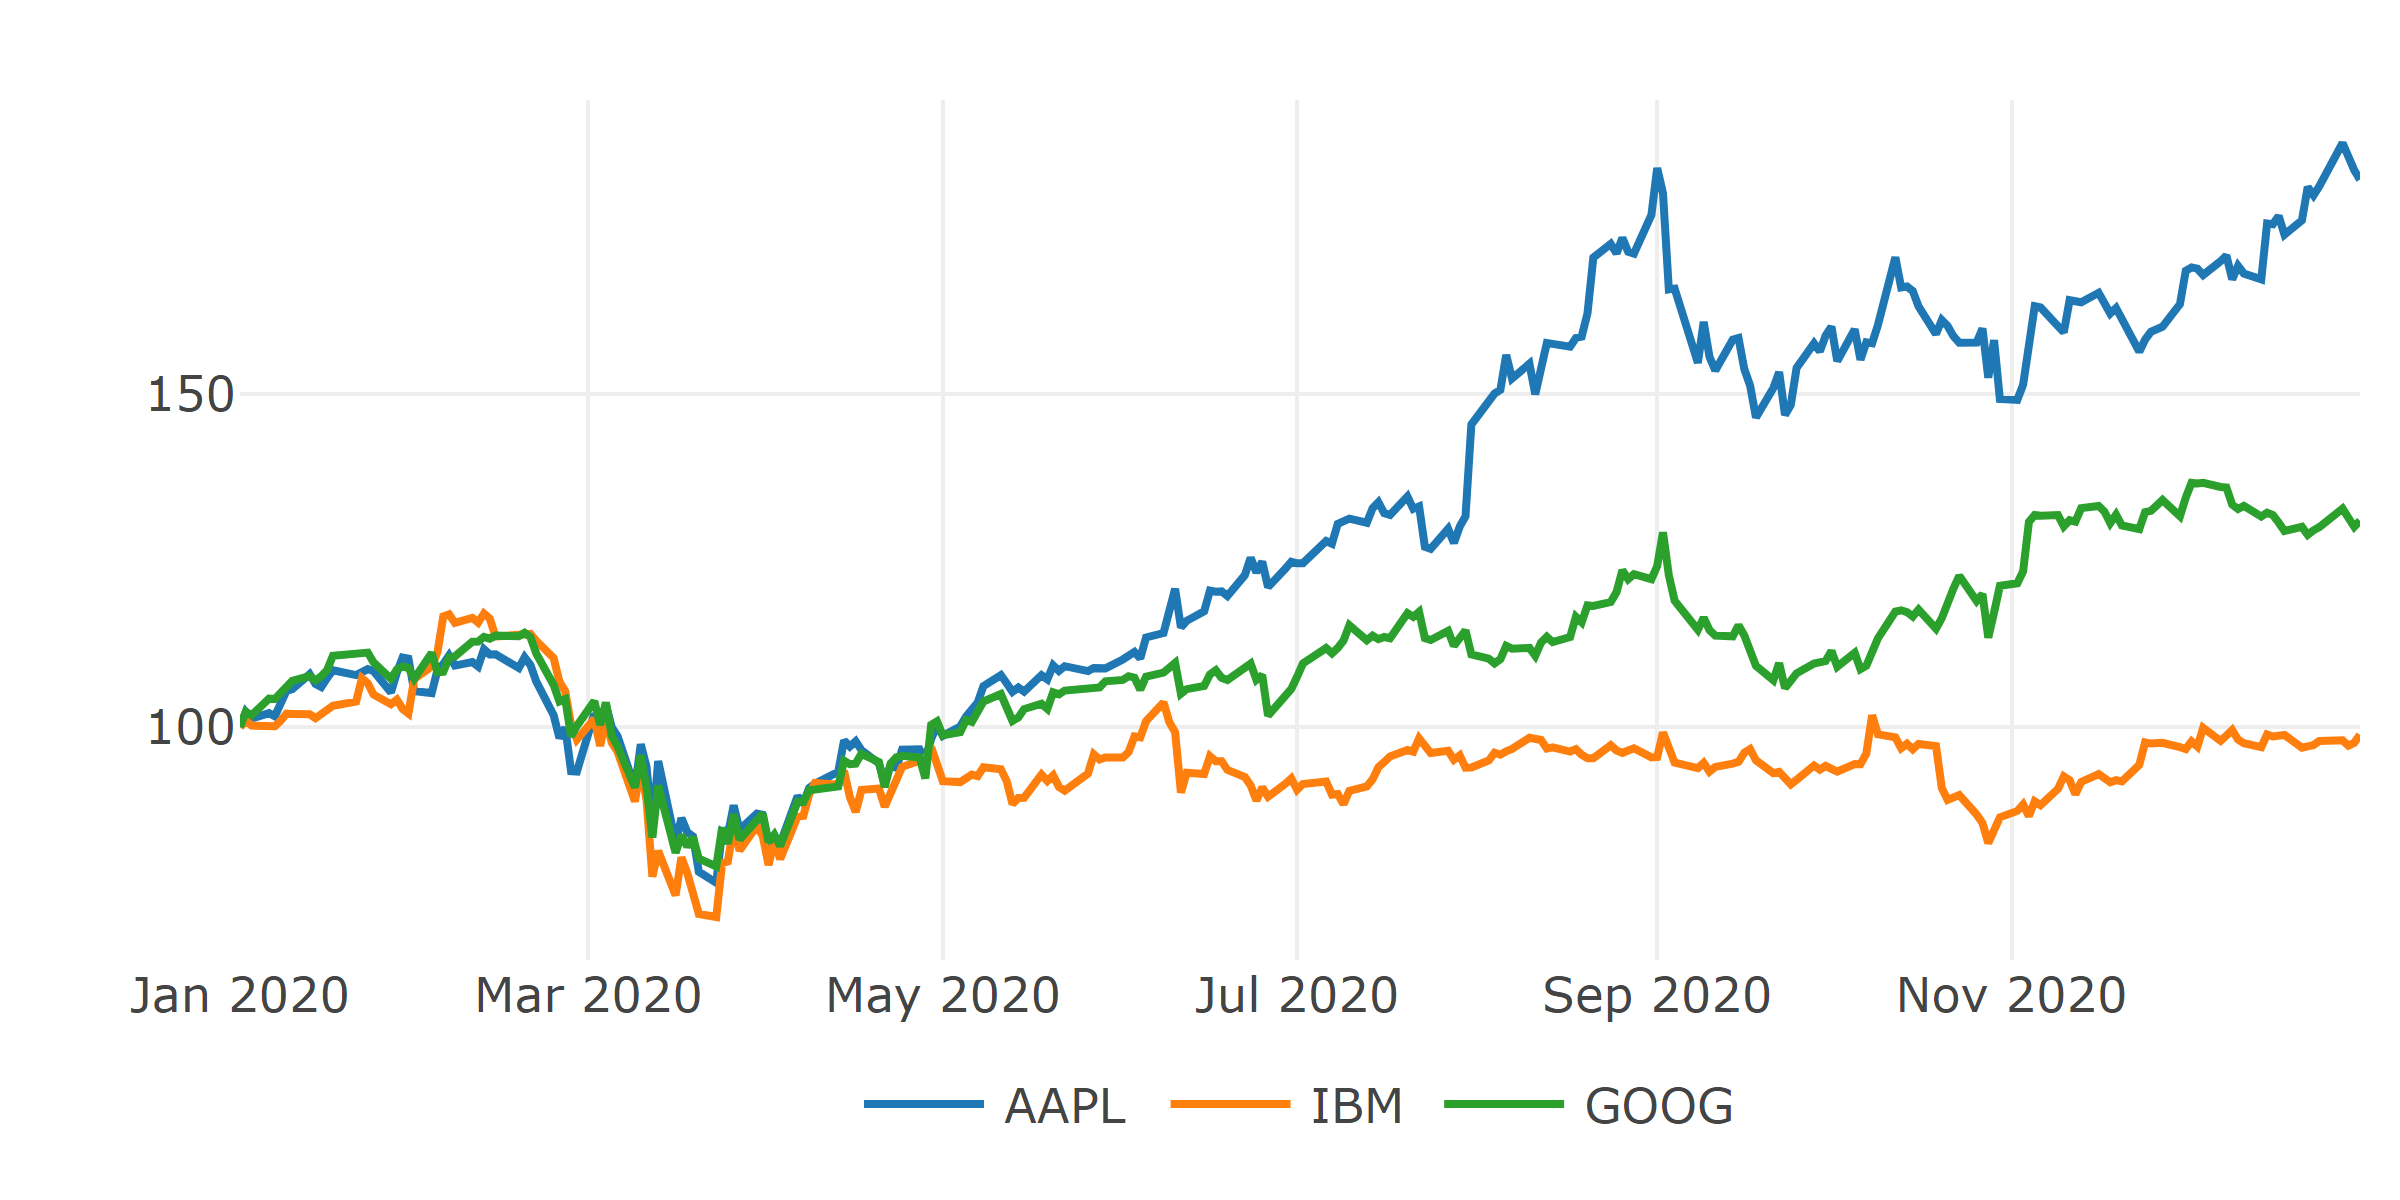
\includegraphics{Master_Thesis_files/figure-latex/unnamed-chunk-3-1.png}

\hypertarget{return-calculation}{%
\section{Return Calculation}\label{return-calculation}}

Any portfolio optimization strategy based on historical data must start with returns. These returns are calculated using \href{https://www.investopedia.com/terms/a/adjusted\%20closing\%20price.asp}{adjusted closing prices}, which show the percentage change over time. Adjusted closing prices are reflecting dividends and are cleaned of by stock splits and rights offerings. These Returns are essential for comparing assets and for analyzing dependencies.

\hypertarget{simple-returns}{%
\subsection{Simple Returns}\label{simple-returns}}

The default timeframe for all raw data in this thesis is one workday and only simple returns are used. Suppose there is a asset with prices \(P\) on workday \(t_i\) and following workday \(t_{i+1}\), then follows that the simple return on \(t_{i+1}\) can be calculated as:
\[
  R_{i+1} = \frac{P_{t_{i+1}}}{P_{t_i}}-1
\]

\hypertarget{markowitz-modern-portfolio-theory-mpt}{%
\section{Markowitz Modern Portfolio Theory (MPT)}\label{markowitz-modern-portfolio-theory-mpt}}

In 1952, Harry Markowitz published his first ground-breaking work, which had a significant influence on modern finance, primarily by outlining the effects of diversification and efficient portfolios. The definition of an efficient portfolio is one that has either the maximum expected return for a given risk target or the minimum risk for a given expected return target. A simple quote to define diversification could be: ``A portfolio has the same return but less variance than the sum of its parts''. This is true if the assets are not perfectly correlated, because bad and good movers can make up for each other which will reduce the likelihood of extreme events. More specific information can be found at \citep{Mari2005}.

\hypertarget{assumptions-of-markowitz-portfolio-theory}{%
\subsection{Assumptions of Markowitz Portfolio Theory}\label{assumptions-of-markowitz-portfolio-theory}}

The following list contains all Markowitz assumptions according to \citep{Mari2005}:

\begin{itemize}
\tightlist
\item
  Perfect market without taxes or transaction costs.
\item
  Short sales are disallowed.
\item
  Assets are infinitely divisible.
\item
  Expected Returns, Variances and Covariances contain all information.
\item
  Investors are risk-adverse, they will only accept greater risk if they
  are compensated with a higher expected return.
\end{itemize}

The assumption that the returns are normally distributed is not required, but it will be assumed in this case to make the problem simpler. It is obvious that these assumptions are unrealistic in real-life. For more details regarding the requirements for utilizing other distributions, have a look at \citep{Mari2005}.

\hypertarget{portfolio-math}{%
\section{Portfolio Math}\label{portfolio-math}}

Proofs for the fundamental calculations required for portfolio optimization as shown in \citep{Eric2021} will be provided in this section. The returns are presented differently than in most sources, because its the most common data-format used in practice. Suppose there are \(N\) assets that are described by a return vector \(R\) of random variables and a portfolio weight vector \(w\), respectively:
\[
  R = 
  \begin{bmatrix}
    R_{1} & R_{2} & \cdots & R_{N}  
 \end{bmatrix}
 , \ \ 
 w = 
  \begin{bmatrix}
    w_{1} \\ 
    w_{2} \\
    \vdots \\
    w_{N}  
 \end{bmatrix}
\]

In this thesis, each return is simplified to be normal distributed with \(R_i = \mathcal{N}(\mu_i, \sigma_i^2)\). As a result, linear combinations of normally distributed random variables are jointly normal distributed and have a mean, variance, and covariance that can be used to fully describe them.

\hypertarget{expected-returns}{%
\subsection{Expected Returns}\label{expected-returns}}

The following formula can be used to get the expected returns of a vector with normally distributed random variables \(R \in \mathbb{R}^{1\times N}\):
\begin{align*}
  E[R] &=
  \begin{bmatrix}
    E[R_{1}] & E[R_{2}] & \cdots & E[R_{N}]  
 \end{bmatrix}\\
 &=
 \begin{bmatrix}
    \mu_{1} & \mu_{2} & \cdots & \mu_{N} 
 \end{bmatrix}
 =
 \mu
\end{align*}
and \(\mu_i\) can be estimated in R with historical data and the formula for geometric mean returns (also called compound returns). The function to calculate the geometric mean returns from a xts-object can be found in \ref{geomeanret}.

\hypertarget{expected-portfolio-returns}{%
\subsection{Expected Portfolio Returns}\label{expected-portfolio-returns}}

The following equation can be used to get the linear combination of expected returns \(\mu\) and a weighting vector \(w\) (e.g.~portfolio weights):
\begin{align*}
 \mu \times w &=
  \begin{bmatrix}
    E[\mu_{1}] & E[\mu_{2}] & \cdots & E[\mu_{N}]
 \end{bmatrix}
  \times 
  \begin{bmatrix}
    w_{1} \\ 
    w_{2} \\
    \cdots \\
    w_{N}  
 \end{bmatrix} \\
 &=
 E[\mu_{1}] \cdot w_1 + E[\mu_{2}] \cdot w_2 + \cdots + E[\mu_{N}] \cdot w_{N} 
 =
 \mu_P
\end{align*}

\hypertarget{covariance}{%
\subsection{Covariance}\label{covariance}}

The general formula of the covariance matrix \(\textstyle\sum\) of a random vector \(R\) with \(N\) normally distributed elements and \(\sigma_{i,j}\) as correlation of two unique assets is described as:
\begin{align*}
  Cov(R) &= E[(R-\mu)^T \otimes (R-\mu)] \\
  &=   \begin{bmatrix}
    \sigma_1^2 & \sigma_{1,2} & \cdots & \sigma_{1,N} \\
    \sigma_{2, 1} & \sigma_2^2 & \cdots & \sigma_{2, N} \\
    \vdots  & \vdots & \ddots & \vdots \\
    \sigma_{N, 1} & \sigma_{N, 2} & \cdots & \sigma_N^2 \\
 \end{bmatrix}\\
  &=\textstyle\sum
\end{align*}
and can be estimated in R with the base-function \texttt{cov()} and historical data.

\hypertarget{portvar}{%
\subsection{Portfolio Variance}\label{portvar}}

Let \(R\) be a random vector with \(N\) normally distributed elements and \(w\) a weighting vector. Suppose the covariance matrix \(\sum\) of \(R\) is known, then the variance of the linear combination of \(R\) can be calculated as:
\begin{align*}
  Var(R \times w) &= E[(R \times w - \mu \times w)^2] \\
  &= E[((R - \mu) \times w)^2]
\end{align*}

Since \((R - \mu) \times w\) is a scalar, it can be transformed from \(((R - \mu) \times w)^2\) to \(((R - \mu) \times w)^T \cdot ((R - \mu) \times w)\) and results in:
\begin{align*}
  Var(R \times w) &= E[((R - \mu) \cdot w)^T \times ((R - \mu) \times w)]\\ 
  &= E[(w^T \times (R - \mu)^T) \cdot ((R - \mu) \times w)]\\ 
  &= w^T \times E[(R - \mu)^T \otimes (R - \mu)] \times w \\
  &= w^T \times Cov(R) \times w \\
  &= w^T \times \textstyle\sum \times w
\end{align*}

The same holds for a estimation of \(\textstyle\sum\).

\hypertarget{portfolioreturns}{%
\subsection{Portfolio Returns}\label{portfolioreturns}}

Suppose there are \(N\) assets which create a portfolio with weights \(w\) at time \(t_0\) and the portfolio should perform multiple timesteps till \(t_T\) without re-balancing. What are the portfolio returns on each timestep \(t_i\)? Its obvious that assets with a positive performance at the current timestep have a higher weight at the next timestep. This can be done by adjusting the weights after each timestep, dependent on the returns. The formula for holding a portfolio with weights \(\textstyle\sum w = 1\) and return matrix \(R \in R^{T \times N}\), has the return \(Z_i-1\) on \(t_i\) with \(i=0, 1, \cdots, T\) for:
\[
  Z_i =
  \left\{
  \begin{split}
  &(1+R_i)\cdot w, &\text{ if }i=0\\
  &(1+R_i)\cdot \frac{Z_{i-1}}{\sum Z_{i-1}}, &\text{ if }i>0
  \end{split}
  \right.
\]
This calculation of portfolio returns is implemented in the \texttt{calc\_portfolio\_returns()} function below.

\hypertarget{r-functions-2}{%
\section{R-Functions}\label{r-functions-2}}

asdad

\hypertarget{pritoret}{%
\subsection{\texorpdfstring{\texttt{pri\_to\_ret()}}{pri\_to\_ret()}}\label{pritoret}}

asdasdasd ((prices to returns))

\hypertarget{ret_to_cumret}{%
\subsection{\texorpdfstring{\texttt{ret\_to\_cumret()}}{ret\_to\_cumret()}}\label{ret_to_cumret}}

asdasdasdasdasd ((returns to cumulated returns normalized to 100))

\hypertarget{geomeanret}{%
\subsection{\texorpdfstring{\texttt{ret\_to\_geomeanret()}}{ret\_to\_geomeanret()}}\label{geomeanret}}

Geometric mean returns are a better estimator than the arithmetic mean returns, because they capture the exact mean price changes over a period of time. Because the estimation of the variance is calculated as daily variance, it needs to do the same with returns over time. This can be done by calculating geometric mean returns from multiple daily returns. Suppose there is an asset with returns \(r_1 = 0.01\), \(r_2=0.03\) and \(r_3=0.02\) then follows that the geometric mean return \(r^{id}\) can be calculated as:
\[
  r^{id} = ((1+r_1) \cdot (1+r_2) \cdot (1+r_3))^{1/3}-1 = 0.01996732
\]
And the benefit is that it's a daily mean return, which will produce exactly the same outcome as the real returns, that means:
\[
  (1+r^{id})^3 = (1+r_1) \cdot (1+r_2) \cdot (1+r_3)
\]
This isnt the case for arithmetic mean returns. The general formula to calculate the mean geometric return from \(n\) days is:
\[
  r^{id} = (\prod_{i=1}^n (1+r_i))^{\frac{1}{n}}-1
\]
and as R-code:

\begin{Shaded}
\begin{Highlighting}[]
\NormalTok{ret\_to\_geomeanret }\OtherTok{\textless{}{-}} \ControlFlowTok{function}\NormalTok{(xts\_ret)\{}
  \FunctionTok{sapply}\NormalTok{((}\DecValTok{1}\SpecialCharTok{+}\NormalTok{xts\_ret), prod)}\SpecialCharTok{\^{}}\NormalTok{(}\DecValTok{1}\SpecialCharTok{/}\FunctionTok{nrow}\NormalTok{(xts\_ret))}\SpecialCharTok{{-}}\DecValTok{1}
\NormalTok{\}}
\end{Highlighting}
\end{Shaded}

\hypertarget{calc_portfolio_returns}{%
\subsection{\texorpdfstring{\texttt{calc\_portfolio\_returns()}}{calc\_portfolio\_returns()}}\label{calc_portfolio_returns}}

This is the implementation of a vectorial calculation of portfolio returns over multiple periods with a weighting vector \texttt{weights} at \(t_0\) and no re-balancing:

\begin{Shaded}
\begin{Highlighting}[]
\NormalTok{calc\_portfolio\_returns }\OtherTok{\textless{}{-}} 
  \ControlFlowTok{function}\NormalTok{(xts\_returns, weights, }\AttributeTok{name=}\StringTok{"portfolio"}\NormalTok{)\{}
  \ControlFlowTok{if}\NormalTok{(}\FunctionTok{sum}\NormalTok{(weights)}\SpecialCharTok{!=}\DecValTok{1}\NormalTok{)\{}
\NormalTok{    xts\_returns}\SpecialCharTok{$}\NormalTok{temp\_\_\_X1 }\OtherTok{\textless{}{-}} \DecValTok{0}
\NormalTok{    weights }\OtherTok{\textless{}{-}} \FunctionTok{c}\NormalTok{(weights, }\DecValTok{1}\SpecialCharTok{{-}}\FunctionTok{sum}\NormalTok{(weights))}
\NormalTok{  \}}
\NormalTok{  res }\OtherTok{\textless{}{-}} \FunctionTok{cumprod}\NormalTok{((}\DecValTok{1}\SpecialCharTok{+}\NormalTok{xts\_returns)) }\SpecialCharTok{*} \FunctionTok{matrix}\NormalTok{(}
    \FunctionTok{rep}\NormalTok{(weights, }\FunctionTok{nrow}\NormalTok{(xts\_returns)), }\AttributeTok{ncol=}\FunctionTok{length}\NormalTok{(weights), }\AttributeTok{byrow=}\NormalTok{T)}
\NormalTok{  res }\OtherTok{\textless{}{-}} \FunctionTok{xts}\NormalTok{(}
    \FunctionTok{rowSums}\NormalTok{(res}\SpecialCharTok{/}\FunctionTok{c}\NormalTok{(}\DecValTok{1}\NormalTok{, }\FunctionTok{rowSums}\NormalTok{(res[}\SpecialCharTok{{-}}\FunctionTok{nrow}\NormalTok{(xts\_returns),])))}\SpecialCharTok{{-}}\DecValTok{1}\NormalTok{, }
    \AttributeTok{order.by=}\FunctionTok{index}\NormalTok{(xts\_returns)) }\SpecialCharTok{\%\textgreater{}\%} 
    \FunctionTok{setNames}\NormalTok{(., name)}
  \FunctionTok{return}\NormalTok{(res)}
\NormalTok{\}}
\end{Highlighting}
\end{Shaded}

This function has the same results as the \texttt{Return.portfolio()} function from the \texttt{PortfolioAnalytics} package.

\hypertarget{activ-vs-passiv-investing}{%
\chapter{Activ vs Passiv Investing}\label{activ-vs-passiv-investing}}

The fundation of Asset Management

passiv vs activ studie
\texttt{https://www.scirp.org/journal/paperinformation.aspx?paperid=92983}

gut gut
\url{file:///C:/Users/Axel/Desktop/Master-Thesis-All/Ziel\%20was\%20beantwortet\%20werden\%20soll/Quellen\%20nur\%20wichtige/Rasmussen2003_Book_QuantitativePortfolioOptimisat.pdf}

\hypertarget{challenges}{%
\chapter{Challenges of Passiv Investing}\label{challenges}}

This Chapter will analyse two common challenges of Passiv-Investing and creates simple use-cases to test the PSO. The first one is the mean-variance portfolio (MVP) from the modern portfolio theory of Markowitz which is simply said an optimal allocation of assets regarding risk and return. The second challenge is the index-tracking-problem which tries to construct a portfolio with minimal tracking error to a given benchmark.

\hypertarget{mean-variance-portfolio-mvp}{%
\section{Mean-Variance Portfolio (MVP)}\label{mean-variance-portfolio-mvp}}

Markowitz has shown that diversifying the risk on multiple assets will reduce the overall risk of the portfolio. This result was the beginning of the widely used modern portfolio theory which uses mathematical models to archive portfolios with minimal variance for a given return target. All these optimal portfolios for a given return target are called efficient and create the efficient frontier.

\hypertarget{mvp}{%
\subsection{MVP}\label{mvp}}

Let there be \(N\) assets and its returns on \(T\) different days which creates a return matrix \(R \in \mathbb{R}^{T \times N}\). Each element \(R_{t,i}\) contains the return of the \(i\)-th asset on day \(t\). The covariance matrix of the returns is \(\textstyle\sum \in \mathbb{R}^{N \times N}\) and the expected returns are \(\mu \in \mathbb{R}^{N}\). The MVP with risk aversion parameter \(\lambda \in [0,1]\) like shown in \citep{Mari2005} can be formalized as follows:
\begin{equation} 
\underset{w}{minimize} \ \ \ \lambda \ w^T \textstyle\sum w - (1-\lambda) \ \mu^T w
\label{eq:MVP}
\end{equation}

The risk aversion parameter \(\lambda\) defines the trade-off between risk and return. With \(\lambda = 1\), the minimization problem only contains the variance term and so on results in a minimum variance portfolio and \(\lambda = 0\) transforms the problem into a minimization of the negative expected returns, which results in a maximum return portfolio. All possible portfolios created by \(\lambda \in [0, 1]\) define the efficient frontier.

\hypertarget{mvp-example}{%
\subsection{MVP example}\label{mvp-example}}

All possible MVPs combined create the efficient frontier, that is analyzed in this section without going into the details of its calculation. This example uses three assets (equitys: IBM, Google, Apple) and calculates the solution of the MVP for each \(\lambda\). First of all are the daily returns of these three assets are loaded from the year 2020.

The cummulated daily returns are:

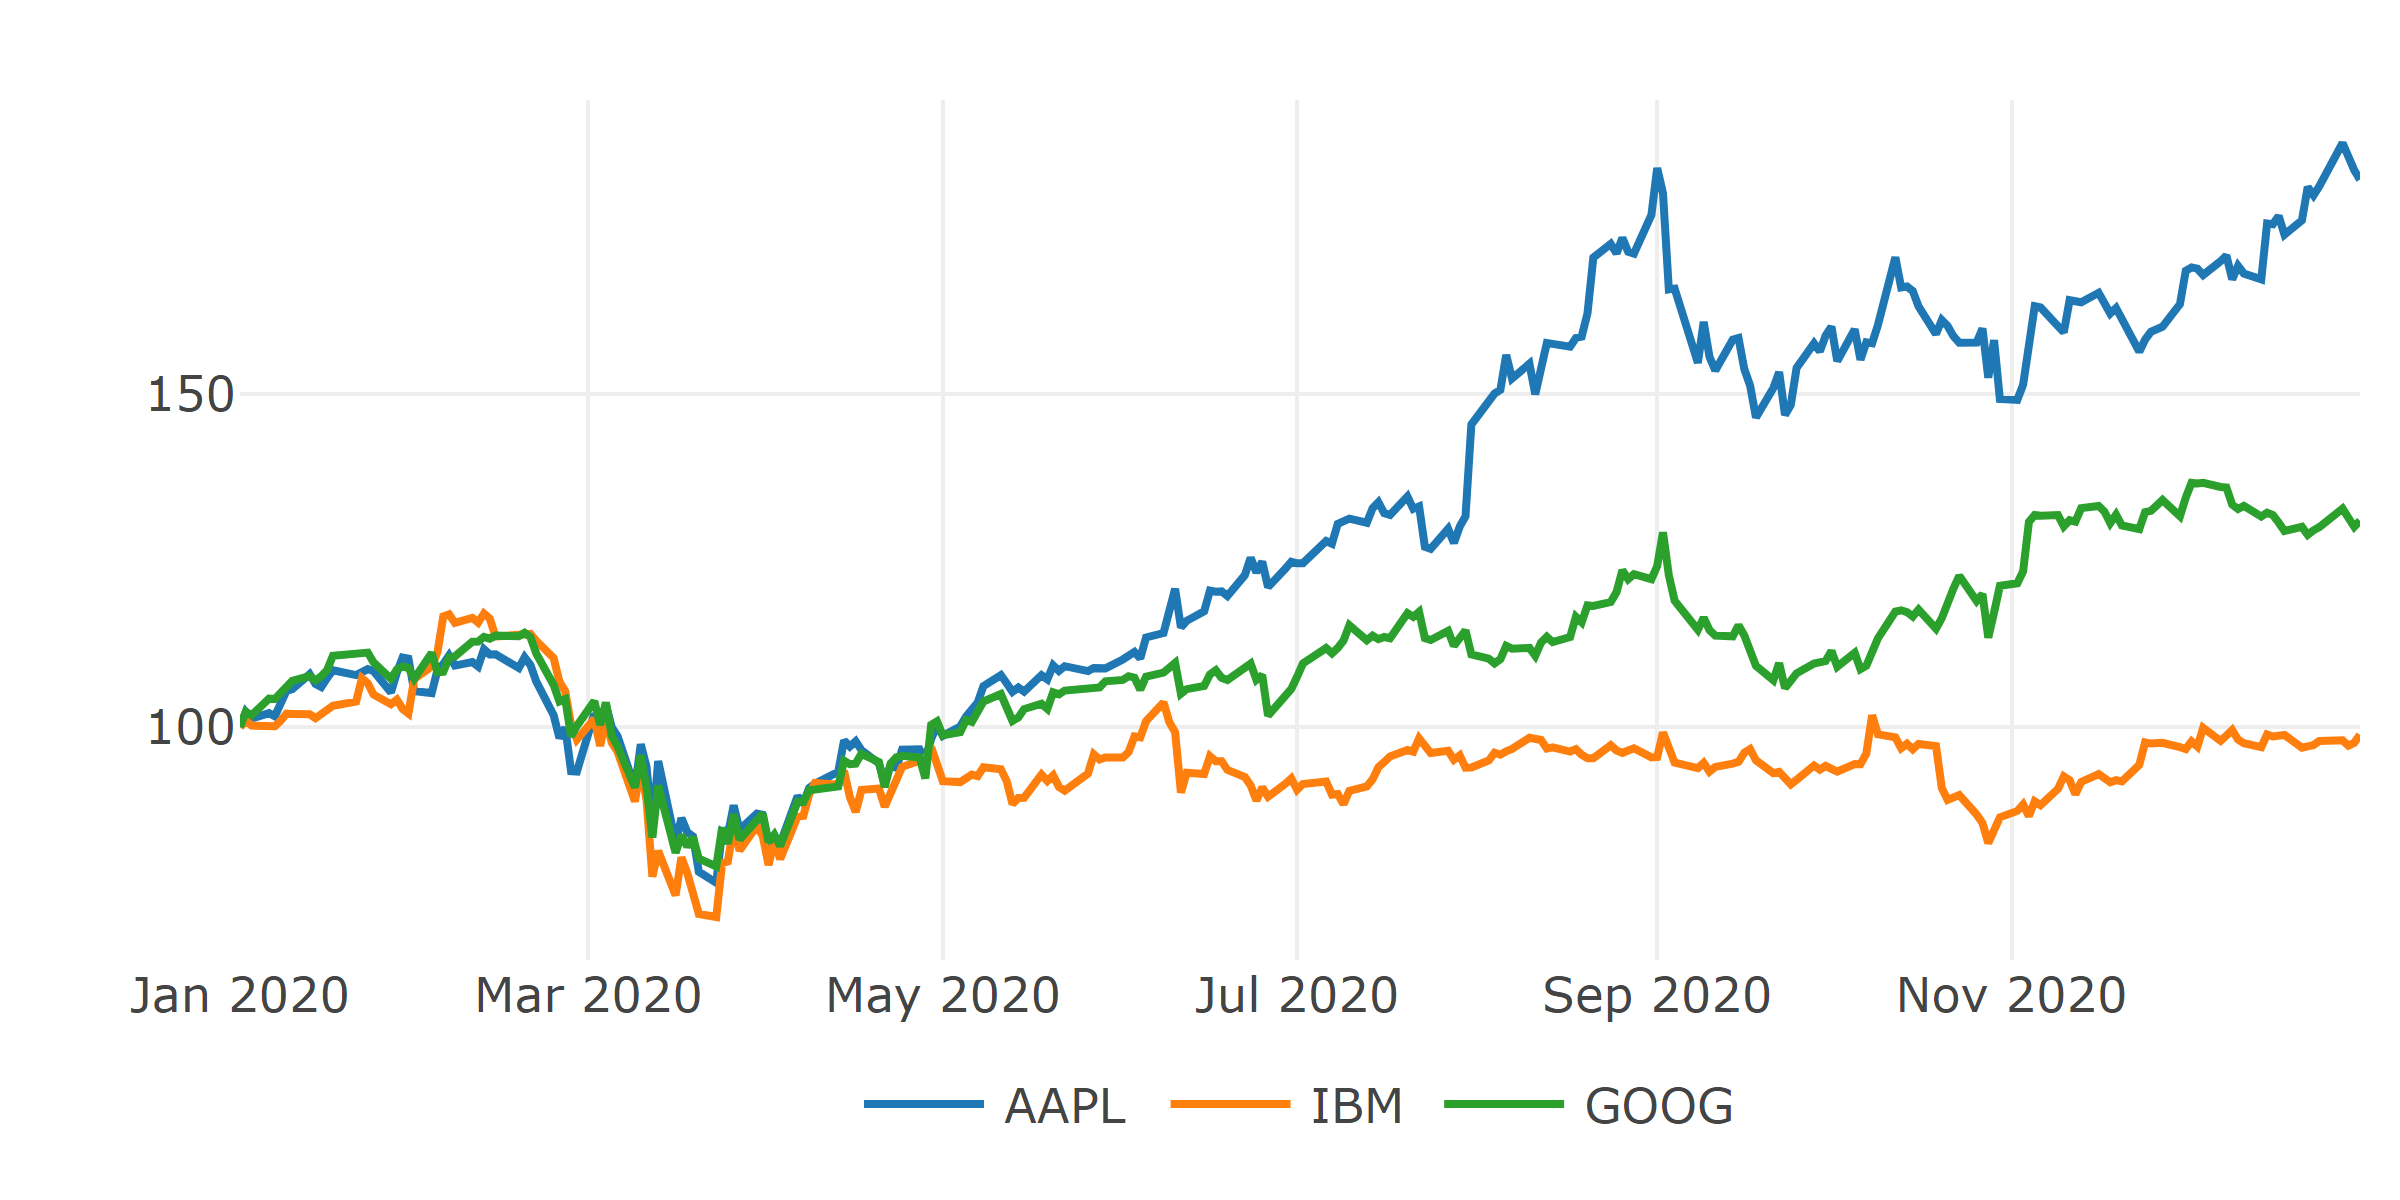
\includegraphics{Master_Thesis_files/figure-latex/unnamed-chunk-7-1.png}

The expected daily returns and the covariance matrix for the 3 assets can be estimated with the formulas from chapter \ref{mathfundations}:

These are all the necessary data to solve the MVP with \(\lambda \in \{0.01, 0.02, ..., 0.99, 1\}\). All 100 portfolios are calculated by solving a quadratic minimization problem with long only constraint and the weights should sum up to 1.

The resulting daily returns and standard deviation are transformed to annual returns and standard deviation and are plotted to create the efficient frontier:

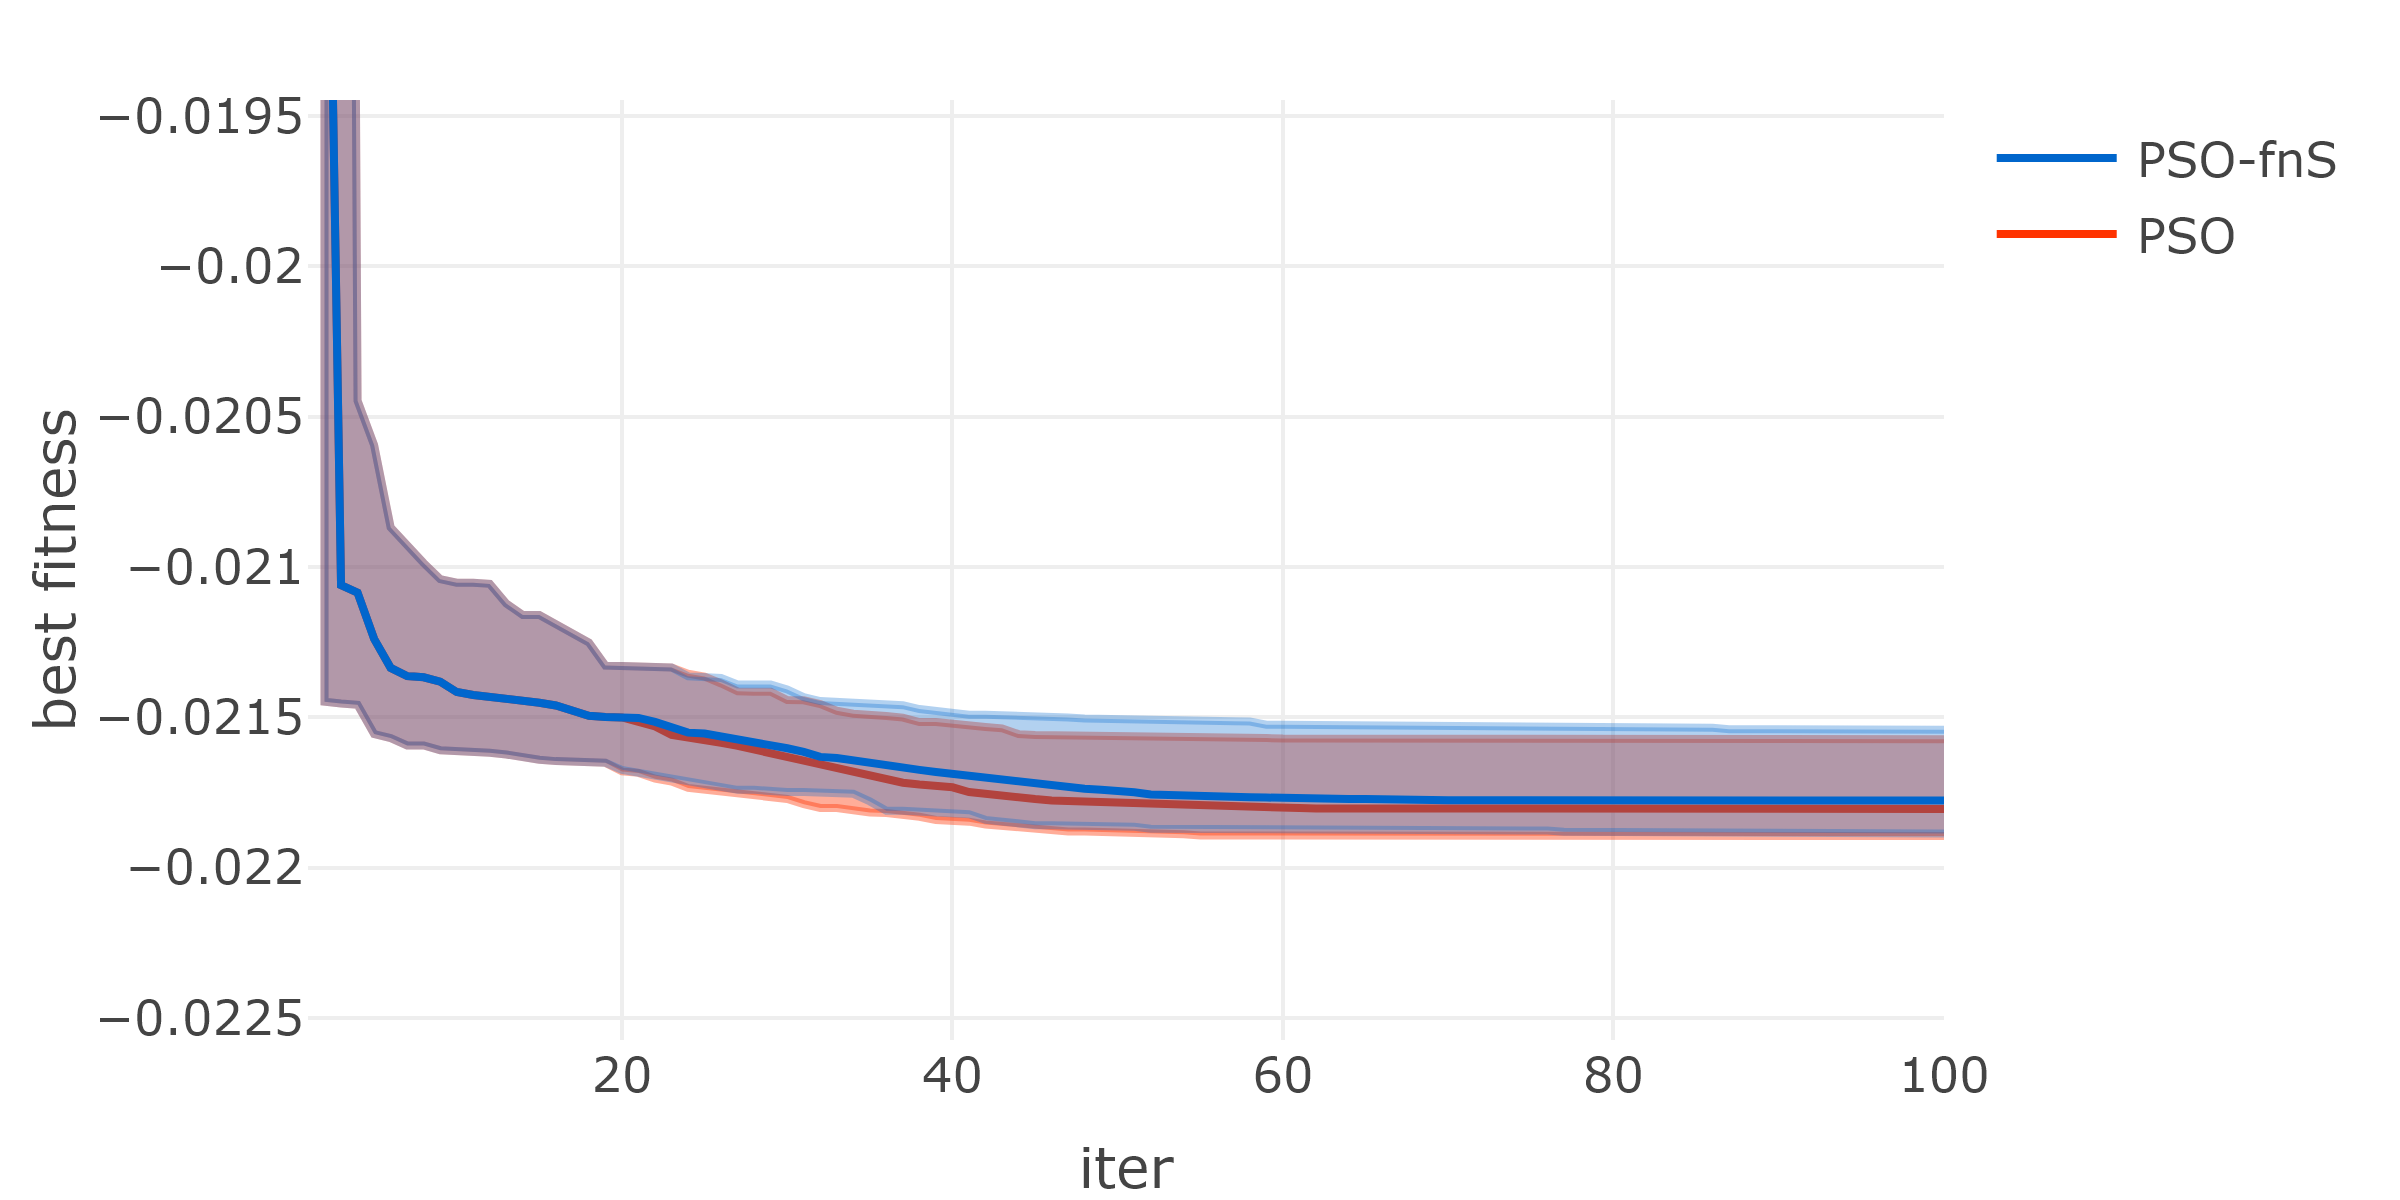
\includegraphics{Master_Thesis_files/figure-latex/unnamed-chunk-10-1.png}

The portfolio compositions for each \(\lambda\)'s are:

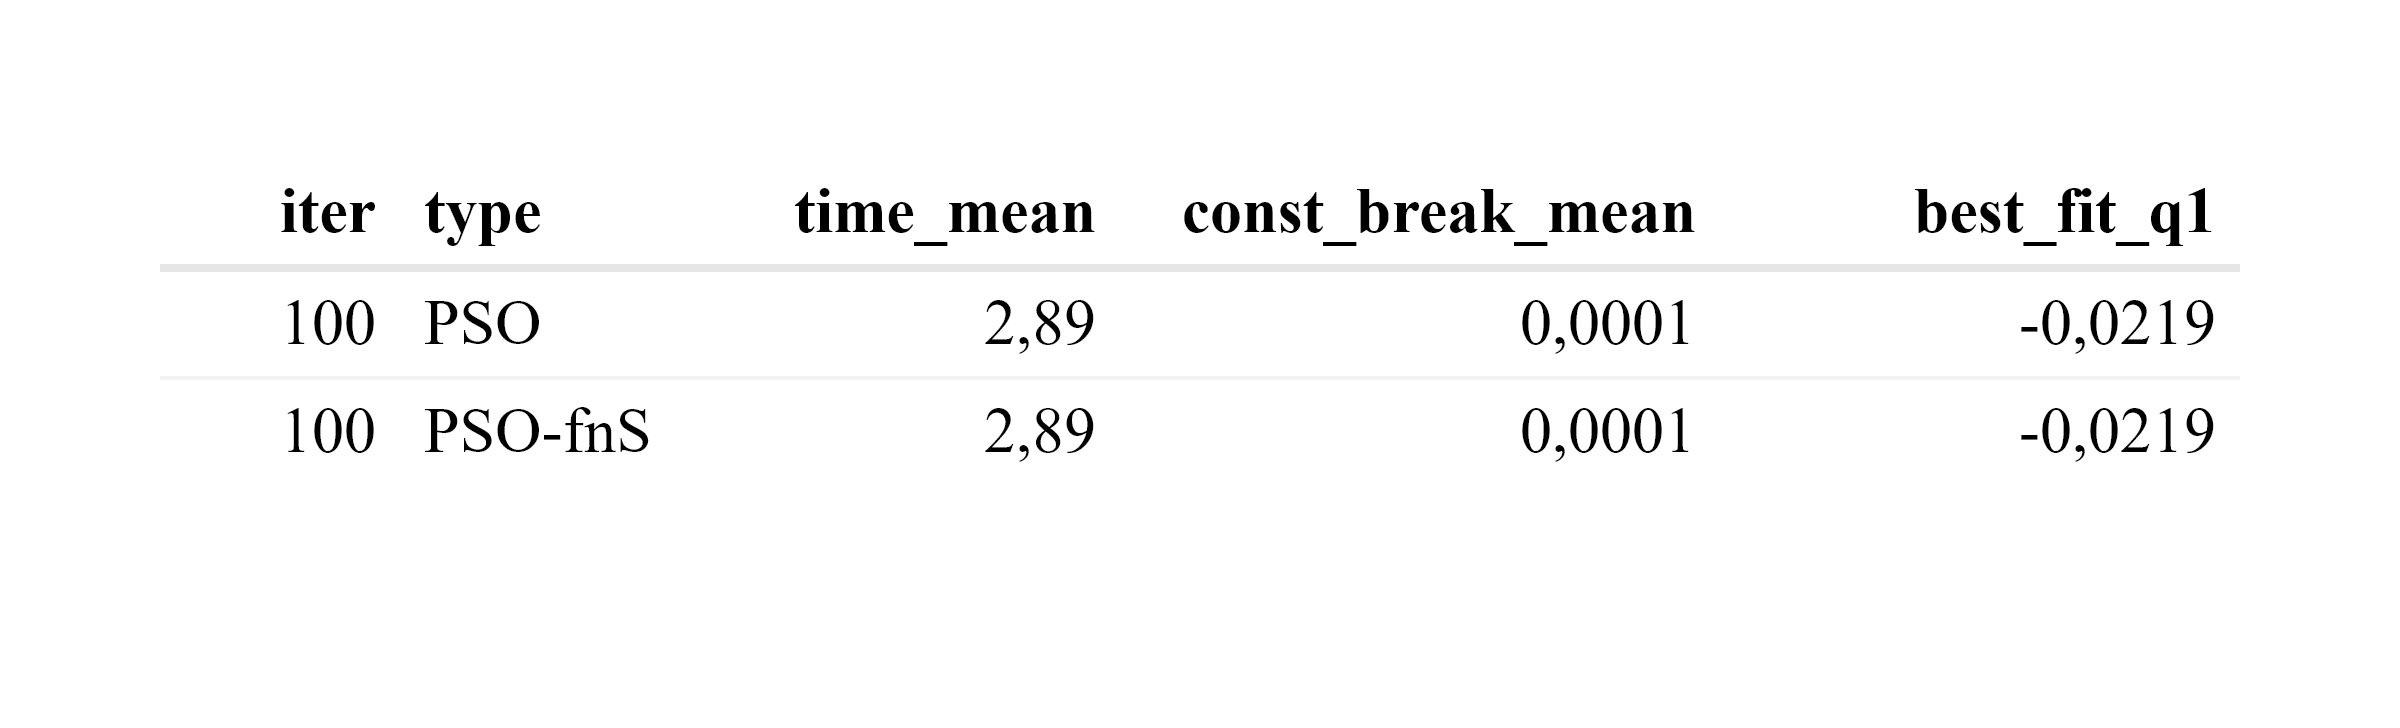
\includegraphics{Master_Thesis_files/figure-latex/unnamed-chunk-11-1.png}

\hypertarget{index-tracking-portfolio-itp}{%
\section{Index-Tracking Portfolio (ITP)}\label{index-tracking-portfolio-itp}}

Indices are baskets of assets that are used to track the performance of a specific asset group. For example, the well-known Standard and Poor's 500 index (short: S\&P 500), tracks the 500 largest companies in the United States. Indices are not purchasable and only serve to visualize the performance of there asset group, without incurring transaction costs. Such indices, or a combination of indices, are used by asset managers as benchmarks to compare the performance of their funds. Each fund has its own benchmark, which contains roughly the same assets that the manager could purchase. If the fund underperforms its benchmark, it may be an indication that the fund manager made poor decisions. That is why fund managers strive to outperform their benchmarks through carefully chosen investments. The past has proven that this is rarely achieved with active management after costs \citep{Desm2016}. This resulted in a growing popularity of passive managed funds with its goal to track there benchmarks as close as possible. It can be accomplished through either full or sparse replication. A full replication is a portfolio that has all assets contained in the benchmark, with the same weights. The resulting performance with neglecting transaction costs, would be exactly the benchmark performance. The first problem is that a benchmark can contain inliquid or not purchasable assets. The second problem would be the weighting scheme of indices, because they are often weighted by its market capitalization which will change daily. This would result in daily work of rebalancing and increasing transaction costs to mimic the benchmarks performance as close as possible. To prevent this, sparse replications are used, that contain a fraction of its benchmarks assets. To do so, the portfolio manager must define his benchmark, which should overlap with his fund's investment universe. Following that, he will reduce this universe using the investors constraints and availability, to create a pool of possible assets. A example pool to track the S\&P 500 could consist of the top hundred highest weighted assets in the S\&P 500. Now is the time to optimize a portfolio with the goal of matching the benchmark performance and taking into account the investors constraints like ratings, asset sectors and more. Typically, this is accomplished by lowering the variance between the portfolio and benchmark returns:

\[
 minimize \ \ Var(r_{p}-r_{bm})
\]

To obtain the portfolio weights \(w\), its necessary to substitute \(r_{p}\) as shown below:

\[
  r_{p} = R \times w
\]

The Variance is then solved up until a quadratic problem dependent on the portfolio weights \(w\) is represented:

\begin{align*}
 Var(r_{p}-r_{bm}) &= Var(R \times w - r_{bm}) \\
 &= Var(R \times w) + Var(r_{bm}) - 2 \cdot Cov(R \times w,r_{bm}) 
\end{align*}

Now the three terms can be solved, beginning with the easiest.

\[
Var(r_{bm}) = \sigma_{bm}^2 = constant
\]

The variance of the portfolio can be solved with \ref{portvar}:

\[
Var(R \times w) = w^T \times Cov(R) \times w
\]
And the last term can be solved the same way as in \citep{Eric2021}:

\begin{align*}
  Cov(A \times a, b) &= Cov(b, A \times a) \\
  &= E[(b-\mu_{b})(A \times a-\mu_{A} \times a)] \\
  &= E[(b-\mu_{b})(A-\mu_{A}) \times a] \\
  &= E[(b-\mu_{b})(A-\mu_{A})] \times a \\
  &= Cov(A,b) \times a
\end{align*}

This results in the final formula of the ITP:

\begin{equation}
  \begin{split}
   Var(r_{p}-r_{bm}) & = Var(R \times w - r_{bm}) \\
   & = Var(R \times w) - 2 \cdot Cov(R \times w,r_{bm}) + Var(r_{bm})  \\
   & = w^T \times Cov(R) \times w - 2 \cdot Cov(r_{bm}, R)^T \times w + \sigma_{bm}^2
   \end{split}
   \label{eq:ITP}
\end{equation}

The minimization problem of the ITP in the general structure needed by many optimizers is:

\[
  min(\frac{1}{2} \cdot b^T \times D \times b -d^T \times b)
\]

Minimization problems can ignore constant terms and global stretching coefficients and still find the same minimum. This results in the general substitution of the ITP as follows:

\[
  D = Cov(R)
\]

and

\[
d = Cov(r_{bm}, R)
\]

Its possible to add some basic constraints like in the MVP, to sum up the weights to 1 and being long only.

\hypertarget{example-itp}{%
\subsection{Example ITP}\label{example-itp}}

This example will show the results of tracking the S\&P 500 with a tracking portfolio that can only invest in IBM, Apple and Google. The time frame is the year 2020 and the goal is to minimize the variance between the portfolios and benchmarks historical returns.

\begin{verbatim}
##      AAPL       IBM      GOOG 
## 0.2681058 0.4040352 0.3278591
\end{verbatim}

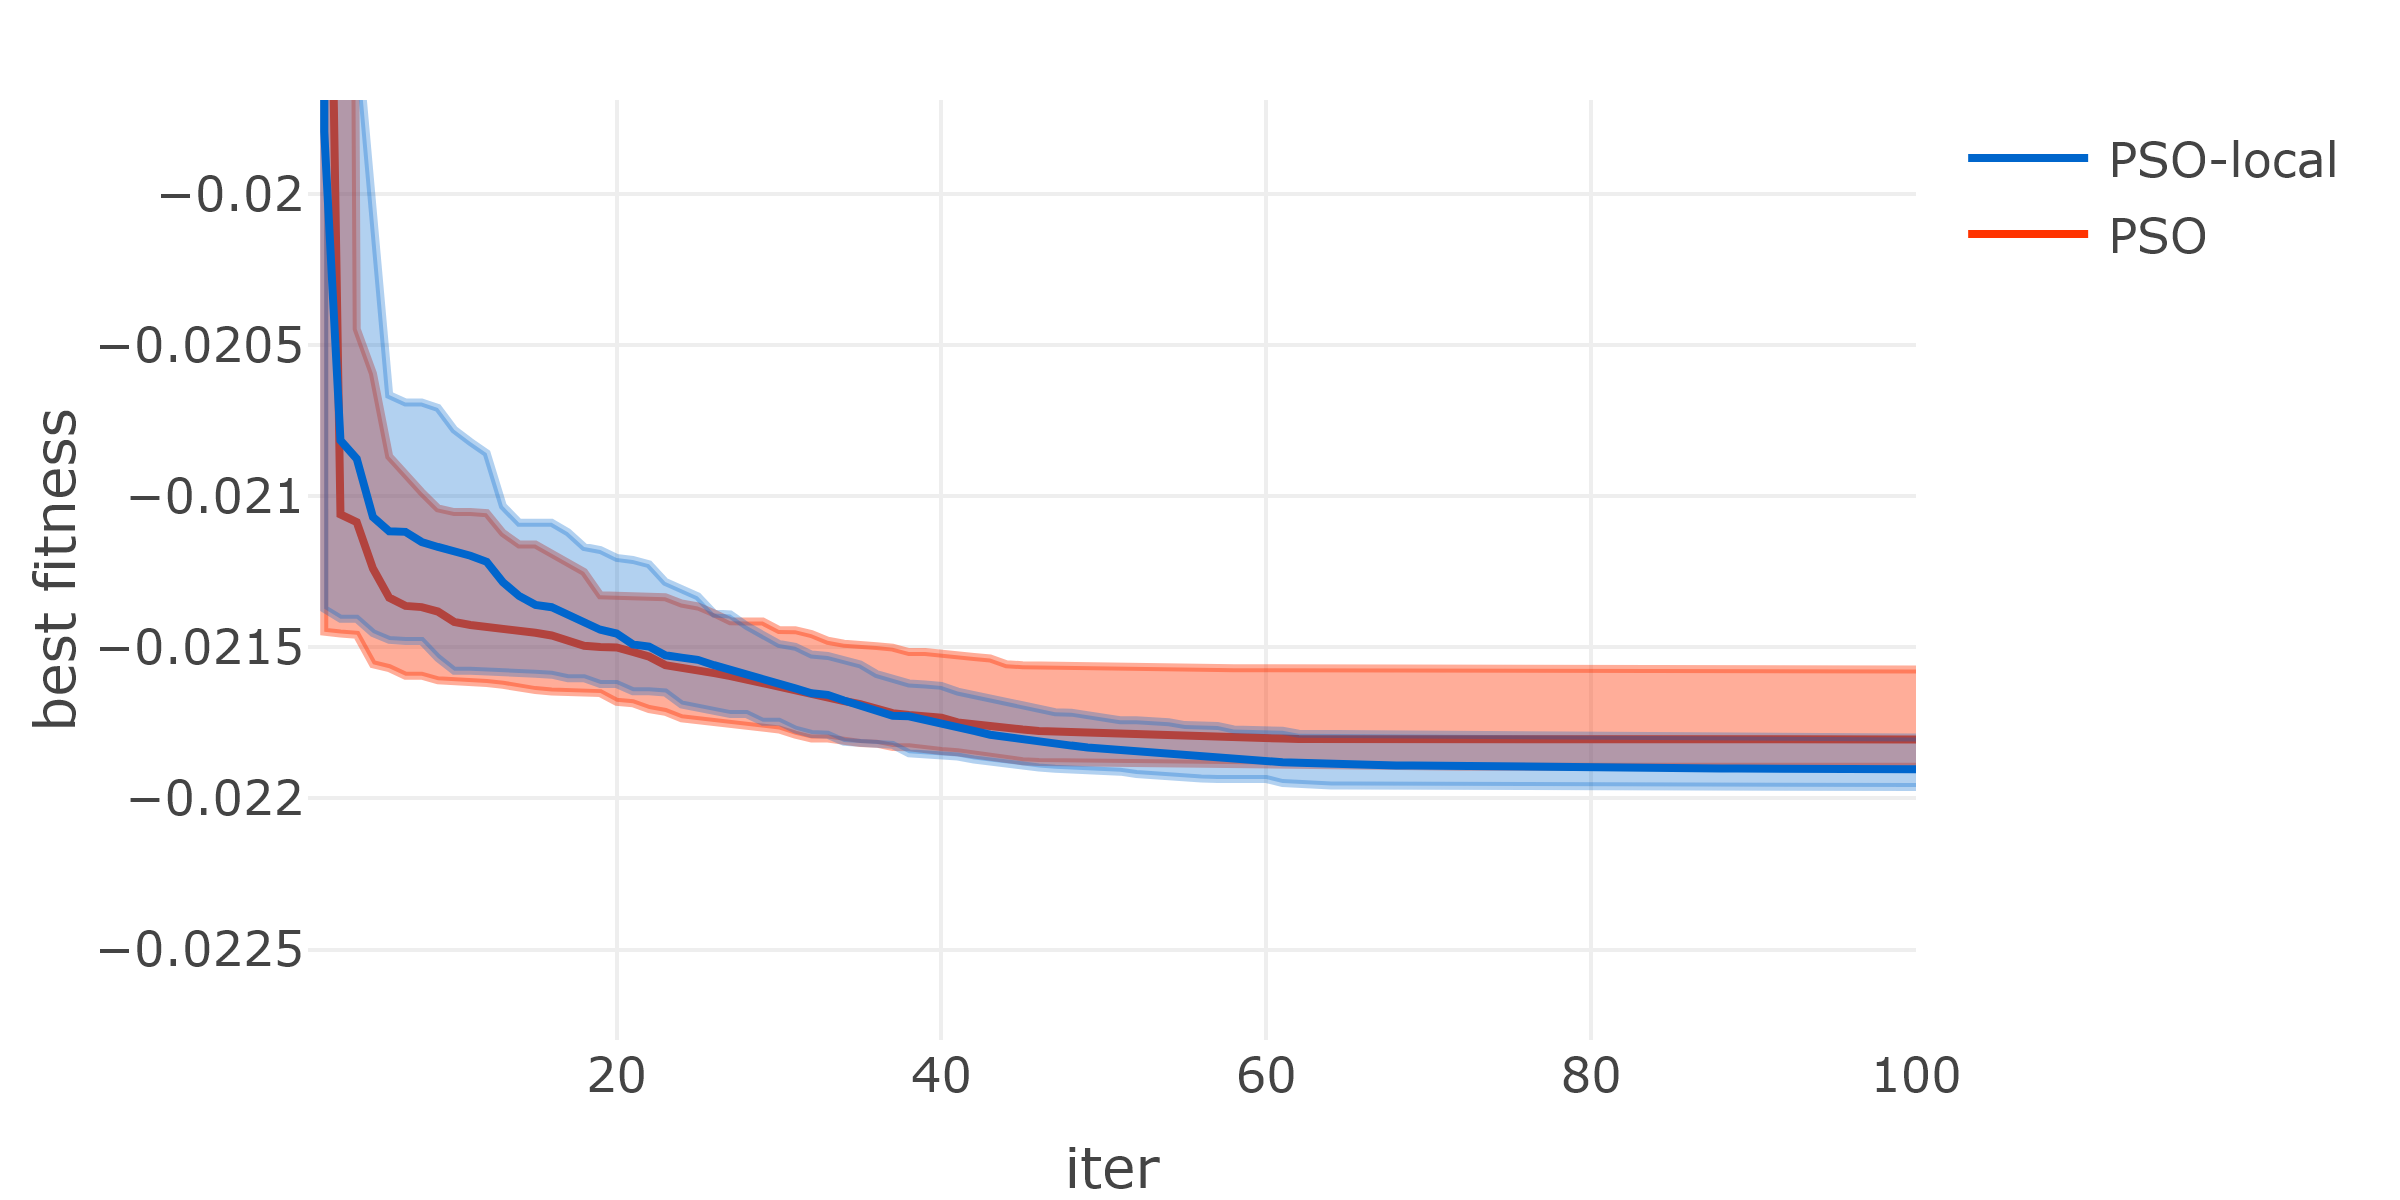
\includegraphics{Master_Thesis_files/figure-latex/unnamed-chunk-12-1.png}

\hypertarget{analytic-solver-for-quadratic-programming-problems}{%
\chapter{Analytic Solver for Quadratic Programming Problems}\label{analytic-solver-for-quadratic-programming-problems}}

The benefits and drawbacks of analytic solvers for quadratic programming problems will be discussed in this chapter. It would go beyond the scope of this thesis to explain the mathematical underlying principles of how a solver addresses quadratic problems, only the applications and analysis are discussed. The foremost reason of addressing quadratic programming solvers is to use it as a benchmark for the PSO.

\hypertarget{quadratic-programming-qp}{%
\section{Quadratic Programming (QP)}\label{quadratic-programming-qp}}

A quadratic program is a minimization problem of some function that returns a scalar and consists of an quadratic term and an linear term, dependent on the variable of interest. Additionally can the problem be constrained by several linear inequalities that restrict the solution. The general formulation used, is to find \(x\) that minimizes the following problem:
\[
  min \ \frac{1}{2} \cdot x^T \times D \times x - d^T \times x 
\]
and holds under the linear constraints:
\[
  A^T \times x >= b_0
\]

Some other sources notate the problem with different signs or coefficients that are all exchangeable with the above stated problem. Additionally has the problem above the same notation that is used in the R-Package \texttt{quadprog} which will reduce substitution efforts. All modern programming languages do have many solvers for quadratic problem. They differ mostly in computational time on specific problems and the requirements. Some commercial QP-solvers do additionally accept more complex constraints, like absolute (e.g.~\(|A^T \times x| >= a_0\)) or mixed-integer (e.g.~\(x \in \mathbb{N}\)). Specially the mixed-integer constraint problems will result in a enormously increase of memory.

\hypertarget{qp-solver-from-quadprog}{%
\section{QP Solver from quadprog}\label{qp-solver-from-quadprog}}

The most common free QP-solver used in R is from the package \href{https://cran.r-project.org/web/packages/quadprog/quadprog.pdf}{quadprog} which consists of a single function named \texttt{solve.QP()}. Its implementation routine is the dual method of Goldfarb and Idnani that was published in \citep{GoId1982} and \citep{GoId1983}. It uses the above stated QP with the requirement that \(D\) needs to be a symmetric positive definite matrix. It means that \(D\in R^{N \times N}\) and \(x^T D x > 0 \ \forall \ x \in R^N\) which is equivalent to, all eigenvalues are bigger than null. In most cases this is not achieved by using the estimation of the covariance matrix \(\sum\), but its possible to find the nearest positive definite matrix of \(\textstyle\sum\) with the function \texttt{nearPD()} from the \href{https://cran.r-project.org/web/packages/Matrix/Matrix.pdf}{Matrix} R-Package. The error that occurs is printed and often do not exceed a percentage change of elements above \(10^{-15} \%\), which is negligible for the context of this thesis. The \texttt{solve.QP()} function for a \(N\) dimensional vector of interest, has the following arguments, that can as well be found in the above stated formulation of a QP:

\begin{itemize}
\tightlist
\item
  \texttt{Dmat}: Symmetric positive definite matrix \(D \in R^{N \times N}\) of the quadratic term.
\item
  \texttt{dvec}: Vector \(d \in R^{N}\) of the linear term
\item
  \texttt{Amat}: Constraint matrix \(A\)
\item
  \texttt{bvec}: Constraint vector \(b_0\)
\item
  \texttt{meq\ =\ 1}: means that the first row of \(A\) is treated as equality constraint
\end{itemize}

The return of \texttt{solve.QP()} is a list and contains among other things the following attributes of interest:

\begin{itemize}
\tightlist
\item
  \texttt{solution}: Vector containing the solution \(x\) of the quadratic programming problem. (e.g.~portfolio weights)
\item
  \texttt{value}: Scalar, the value of the quadratic function at the solution
\end{itemize}

\hypertarget{exampleanalyticalmvp}{%
\section{\texorpdfstring{Example: Solving MVP with \texttt{solve.QP()}}{Example: Solving MVP with solve.QP()}}\label{exampleanalyticalmvp}}

This section provides insights into the effects of diversification and the use of \texttt{solve.QP}, by creating ten different efficient frontiers from a pool of ten assets. Each efficient frontier \(i \in \{1, 2, \cdots, 10\}\) consists of \(N_i = i\) assets and is created by adding the asset with the next smallest variance first. After loading returns for ten of the biggest equity's in the US market, the variance is calculated to arrange all columns ascending by its variance, like shown in the code bellow:

\begin{Shaded}
\begin{Highlighting}[]
\NormalTok{returns\_raw }\OtherTok{\textless{}{-}} \FunctionTok{buffer}\NormalTok{(}
  \FunctionTok{get\_yf}\NormalTok{(}
    \AttributeTok{tickers =} \FunctionTok{c}\NormalTok{(}\StringTok{"IBM"}\NormalTok{, }\StringTok{"GOOG"}\NormalTok{, }\StringTok{"AAPL"}\NormalTok{, }\StringTok{"MSFT"}\NormalTok{, }\StringTok{"AMZN"}\NormalTok{, }
                \StringTok{"NVDA"}\NormalTok{, }\StringTok{"JPM"}\NormalTok{, }\StringTok{"META"}\NormalTok{, }\StringTok{"V"}\NormalTok{, }\StringTok{"WMT"}\NormalTok{), }
    \AttributeTok{from =} \StringTok{"2016{-}01{-}01"}\NormalTok{, }
    \AttributeTok{to =} \StringTok{"2021{-}12{-}31"}
\NormalTok{  )}\SpecialCharTok{$}\NormalTok{returns, }
  \StringTok{"AS\_10\_assets"}
\NormalTok{)}

\CommentTok{\# re{-}arrange: low var first}
\NormalTok{vars }\OtherTok{\textless{}{-}} \FunctionTok{sapply}\NormalTok{(returns\_raw, var)}
\NormalTok{returns\_raw }\OtherTok{\textless{}{-}}\NormalTok{ returns\_raw[, }\FunctionTok{order}\NormalTok{(vars, }\AttributeTok{decreasing =}\NormalTok{ F)]}
\end{Highlighting}
\end{Shaded}

The next step is to create a function \texttt{mvp()} that has the arguments \texttt{return} and \texttt{lambda}. It calculates the expected returns \texttt{mu} and the estimated positive definite covariance \texttt{cov}. Afterwards it solves a MVP with the constraints \(\textstyle\sum w = 1\) and \(w>=0\), which returns key features \texttt{mu}, \texttt{var} and \texttt{composition} of the portfolio.

\begin{Shaded}
\begin{Highlighting}[]
\NormalTok{mvp }\OtherTok{\textless{}{-}} \ControlFlowTok{function}\NormalTok{(returns, lambda)\{}
\NormalTok{  tc }\OtherTok{\textless{}{-}} \FunctionTok{tryCatch}\NormalTok{(\{}
\NormalTok{    mu }\OtherTok{\textless{}{-}} \FunctionTok{sapply}\NormalTok{((}\DecValTok{1}\SpecialCharTok{+}\NormalTok{returns), prod)}\SpecialCharTok{\^{}}\NormalTok{(}\DecValTok{1}\SpecialCharTok{/}\FunctionTok{nrow}\NormalTok{(returns))}\SpecialCharTok{{-}}\DecValTok{1}

\NormalTok{    cov }\OtherTok{\textless{}{-}} \FunctionTok{as.matrix}\NormalTok{(}\FunctionTok{nearPD}\NormalTok{(}\FunctionTok{cov}\NormalTok{(returns))}\SpecialCharTok{$}\NormalTok{mat)}

\NormalTok{    mat }\OtherTok{\textless{}{-}} \FunctionTok{list}\NormalTok{(}
      \AttributeTok{Dmat =}\NormalTok{ lambda }\SpecialCharTok{*}\NormalTok{ cov,}
      \AttributeTok{dvec =}\NormalTok{ (}\DecValTok{1}\SpecialCharTok{{-}}\NormalTok{lambda) }\SpecialCharTok{*}\NormalTok{ mu,}
      \AttributeTok{Amat =} \FunctionTok{t}\NormalTok{(}\FunctionTok{rbind}\NormalTok{(}
        \FunctionTok{rep}\NormalTok{(}\DecValTok{1}\NormalTok{, }\FunctionTok{ncol}\NormalTok{(returns)), }\CommentTok{\# sum up to 1}
        \FunctionTok{diag}\NormalTok{(}\DecValTok{1}\NormalTok{, }\AttributeTok{nrow=}\FunctionTok{ncol}\NormalTok{(returns), }\AttributeTok{ncol=}\FunctionTok{ncol}\NormalTok{(returns)) }\CommentTok{\# long only}
\NormalTok{      )),}
      \AttributeTok{bvec =} \FunctionTok{c}\NormalTok{(}
        \DecValTok{1}\NormalTok{, }\CommentTok{\# sum up to 1}
        \FunctionTok{rep}\NormalTok{(}\DecValTok{0}\NormalTok{, }\FunctionTok{ncol}\NormalTok{(returns)) }\CommentTok{\# long only}
\NormalTok{      ),}
      \AttributeTok{meq =} \DecValTok{1}
\NormalTok{    )}
  
\NormalTok{    qp }\OtherTok{\textless{}{-}} \FunctionTok{solve.QP}\NormalTok{(}
      \AttributeTok{Dmat =}\NormalTok{ mat}\SpecialCharTok{$}\NormalTok{Dmat, }\AttributeTok{dvec =}\NormalTok{ mat}\SpecialCharTok{$}\NormalTok{dvec, }
      \AttributeTok{Amat =}\NormalTok{ mat}\SpecialCharTok{$}\NormalTok{Amat, }\AttributeTok{bvec =}\NormalTok{ mat}\SpecialCharTok{$}\NormalTok{bvec, }\AttributeTok{meq =}\NormalTok{ mat}\SpecialCharTok{$}\NormalTok{meq}
\NormalTok{    )}
    
\NormalTok{    res }\OtherTok{\textless{}{-}} \FunctionTok{list}\NormalTok{(}
      \StringTok{"mu"} \OtherTok{=}\NormalTok{ mu }\SpecialCharTok{\%*\%}\NormalTok{ qp}\SpecialCharTok{$}\NormalTok{solution,}
      \StringTok{"var"} \OtherTok{=} \FunctionTok{t}\NormalTok{(qp}\SpecialCharTok{$}\NormalTok{solution) }\SpecialCharTok{\%*\%}\NormalTok{ cov }\SpecialCharTok{\%*\%}\NormalTok{ qp}\SpecialCharTok{$}\NormalTok{solution,}
      \StringTok{"composition"} \OtherTok{=} \FunctionTok{setNames}\NormalTok{(qp}\SpecialCharTok{$}\NormalTok{solution, }\FunctionTok{colnames}\NormalTok{(returns))}
\NormalTok{    )}
    \ConstantTok{TRUE}
\NormalTok{  \}, }\AttributeTok{error =} \ControlFlowTok{function}\NormalTok{(e)\{}\ConstantTok{FALSE}\NormalTok{\})}
  

  \ControlFlowTok{if}\NormalTok{(tc)\{}
    \FunctionTok{return}\NormalTok{(res)}
\NormalTok{  \}}\ControlFlowTok{else}\NormalTok{\{}
    \FunctionTok{return}\NormalTok{(}\FunctionTok{list}\NormalTok{(}
      \StringTok{"mu"} \OtherTok{=} \ConstantTok{NA}\NormalTok{,}
      \StringTok{"var"} \OtherTok{=} \ConstantTok{NA}\NormalTok{,}
      \StringTok{"composition"} \OtherTok{=} \ConstantTok{NA}
\NormalTok{    ))}
\NormalTok{  \}}
\NormalTok{\}}
\end{Highlighting}
\end{Shaded}

Each \(\lambda \in \{0.01, 0.02, \cdots, 1\}\) and each combination of ascending number of assets produces one portfolio that can be generated with two for loops.

The result gets filtered and names are added that represent the number of assets. Now can the plot be generated:

\begin{Shaded}
\begin{Highlighting}[]
\NormalTok{df }\OtherTok{\textless{}{-}}\NormalTok{ df }\SpecialCharTok{\%\textgreater{}\%} 
  \FunctionTok{filter}\NormalTok{(}\SpecialCharTok{!}\FunctionTok{is.na}\NormalTok{(return)) }\SpecialCharTok{\%\textgreater{}\%} 
  \FunctionTok{distinct}\NormalTok{() }\SpecialCharTok{\%\textgreater{}\%} 
  \FunctionTok{mutate}\NormalTok{(}\AttributeTok{name =} \FunctionTok{paste0}\NormalTok{(}\StringTok{"n\_"}\NormalTok{, index)) }\SpecialCharTok{\%\textgreater{}\%} 
  \FunctionTok{arrange}\NormalTok{(name) }\SpecialCharTok{\%\textgreater{}\%} 
  \FunctionTok{mutate}\NormalTok{(}\AttributeTok{name =} \FunctionTok{factor}\NormalTok{(name, }\AttributeTok{levels=}\FunctionTok{paste0}\NormalTok{(}\StringTok{"n\_"}\NormalTok{, }\FunctionTok{ncol}\NormalTok{(returns\_raw)}\SpecialCharTok{:}\DecValTok{1}\NormalTok{)))}


\NormalTok{max\_show\_sd }\OtherTok{\textless{}{-}}\NormalTok{ df }\SpecialCharTok{\%\textgreater{}\%} 
  \FunctionTok{group\_by}\NormalTok{(index) }\SpecialCharTok{\%\textgreater{}\%} 
  \FunctionTok{summarise}\NormalTok{(}\AttributeTok{max\_x =} \FunctionTok{max}\NormalTok{(var)) }\SpecialCharTok{\%\textgreater{}\%} 
  \FunctionTok{pull}\NormalTok{(max\_x) }\SpecialCharTok{\%\textgreater{}\%} 
  \FunctionTok{mean}\NormalTok{() }\SpecialCharTok{\%\textgreater{}\%} 
  \FunctionTok{sqrt}\NormalTok{()}

\FunctionTok{plot\_ly}\NormalTok{(}
    \AttributeTok{data =}\NormalTok{ df[df}\SpecialCharTok{$}\NormalTok{index}\SpecialCharTok{!=}\DecValTok{1}\NormalTok{,], }
    \AttributeTok{x=}\SpecialCharTok{\textasciitilde{}}\FunctionTok{sqrt}\NormalTok{(var), }
    \AttributeTok{y=}\SpecialCharTok{\textasciitilde{}}\NormalTok{return, }
    \AttributeTok{name=}\SpecialCharTok{\textasciitilde{}}\NormalTok{name, }
    \AttributeTok{mode=}\StringTok{"lines"}\NormalTok{, }
    \AttributeTok{type =} \StringTok{\textquotesingle{}scatter\textquotesingle{}}\NormalTok{, }
    \AttributeTok{color =} \SpecialCharTok{\textasciitilde{}}\NormalTok{name, }
    \AttributeTok{colors =} \FunctionTok{c}\NormalTok{(}\StringTok{"green"}\NormalTok{, }\StringTok{"red"}\NormalTok{)}
\NormalTok{  ) }\SpecialCharTok{\%\textgreater{}\%} 
  \FunctionTok{add\_trace}\NormalTok{(}
    \AttributeTok{data=}\NormalTok{df[df}\SpecialCharTok{$}\NormalTok{index}\SpecialCharTok{==}\DecValTok{1}\NormalTok{,],  }
    \AttributeTok{x=}\SpecialCharTok{\textasciitilde{}}\FunctionTok{sqrt}\NormalTok{(var), }
    \AttributeTok{y=}\SpecialCharTok{\textasciitilde{}}\NormalTok{return, }
    \AttributeTok{showlegend=}\NormalTok{T, }
    \AttributeTok{marker=}\FunctionTok{list}\NormalTok{(}\AttributeTok{color=}\StringTok{"red"}\NormalTok{), }
    \AttributeTok{mode=}\StringTok{"markers"}\NormalTok{, }
    \AttributeTok{name=}\StringTok{"n\_1"}\NormalTok{) }\SpecialCharTok{\%\textgreater{}\%} 
  \FunctionTok{layout}\NormalTok{(}
    \AttributeTok{xaxis=}\FunctionTok{list}\NormalTok{(}\AttributeTok{range=}\FunctionTok{c}\NormalTok{(}\FunctionTok{sqrt}\NormalTok{(}\FunctionTok{min}\NormalTok{(df}\SpecialCharTok{$}\NormalTok{var))}\SpecialCharTok{*}\FloatTok{0.9}\NormalTok{, max\_show\_sd), }\AttributeTok{title=}\StringTok{"standard deviation"}\NormalTok{),}
    \AttributeTok{yaxis=}\FunctionTok{list}\NormalTok{(}\AttributeTok{range=}\FunctionTok{c}\NormalTok{(}\FunctionTok{min}\NormalTok{(df}\SpecialCharTok{$}\NormalTok{return)}\SpecialCharTok{*}\FloatTok{0.9}\NormalTok{, (}\FunctionTok{max}\NormalTok{(df}\SpecialCharTok{$}\NormalTok{return)}\SpecialCharTok{+}\FunctionTok{mean}\NormalTok{(df}\SpecialCharTok{$}\NormalTok{return))}\SpecialCharTok{*}\FloatTok{0.5}\NormalTok{), }\AttributeTok{title=}\StringTok{"return"}\NormalTok{)) }\SpecialCharTok{\%\textgreater{}\%} 
  \FunctionTok{html\_save}\NormalTok{()}
\end{Highlighting}
\end{Shaded}

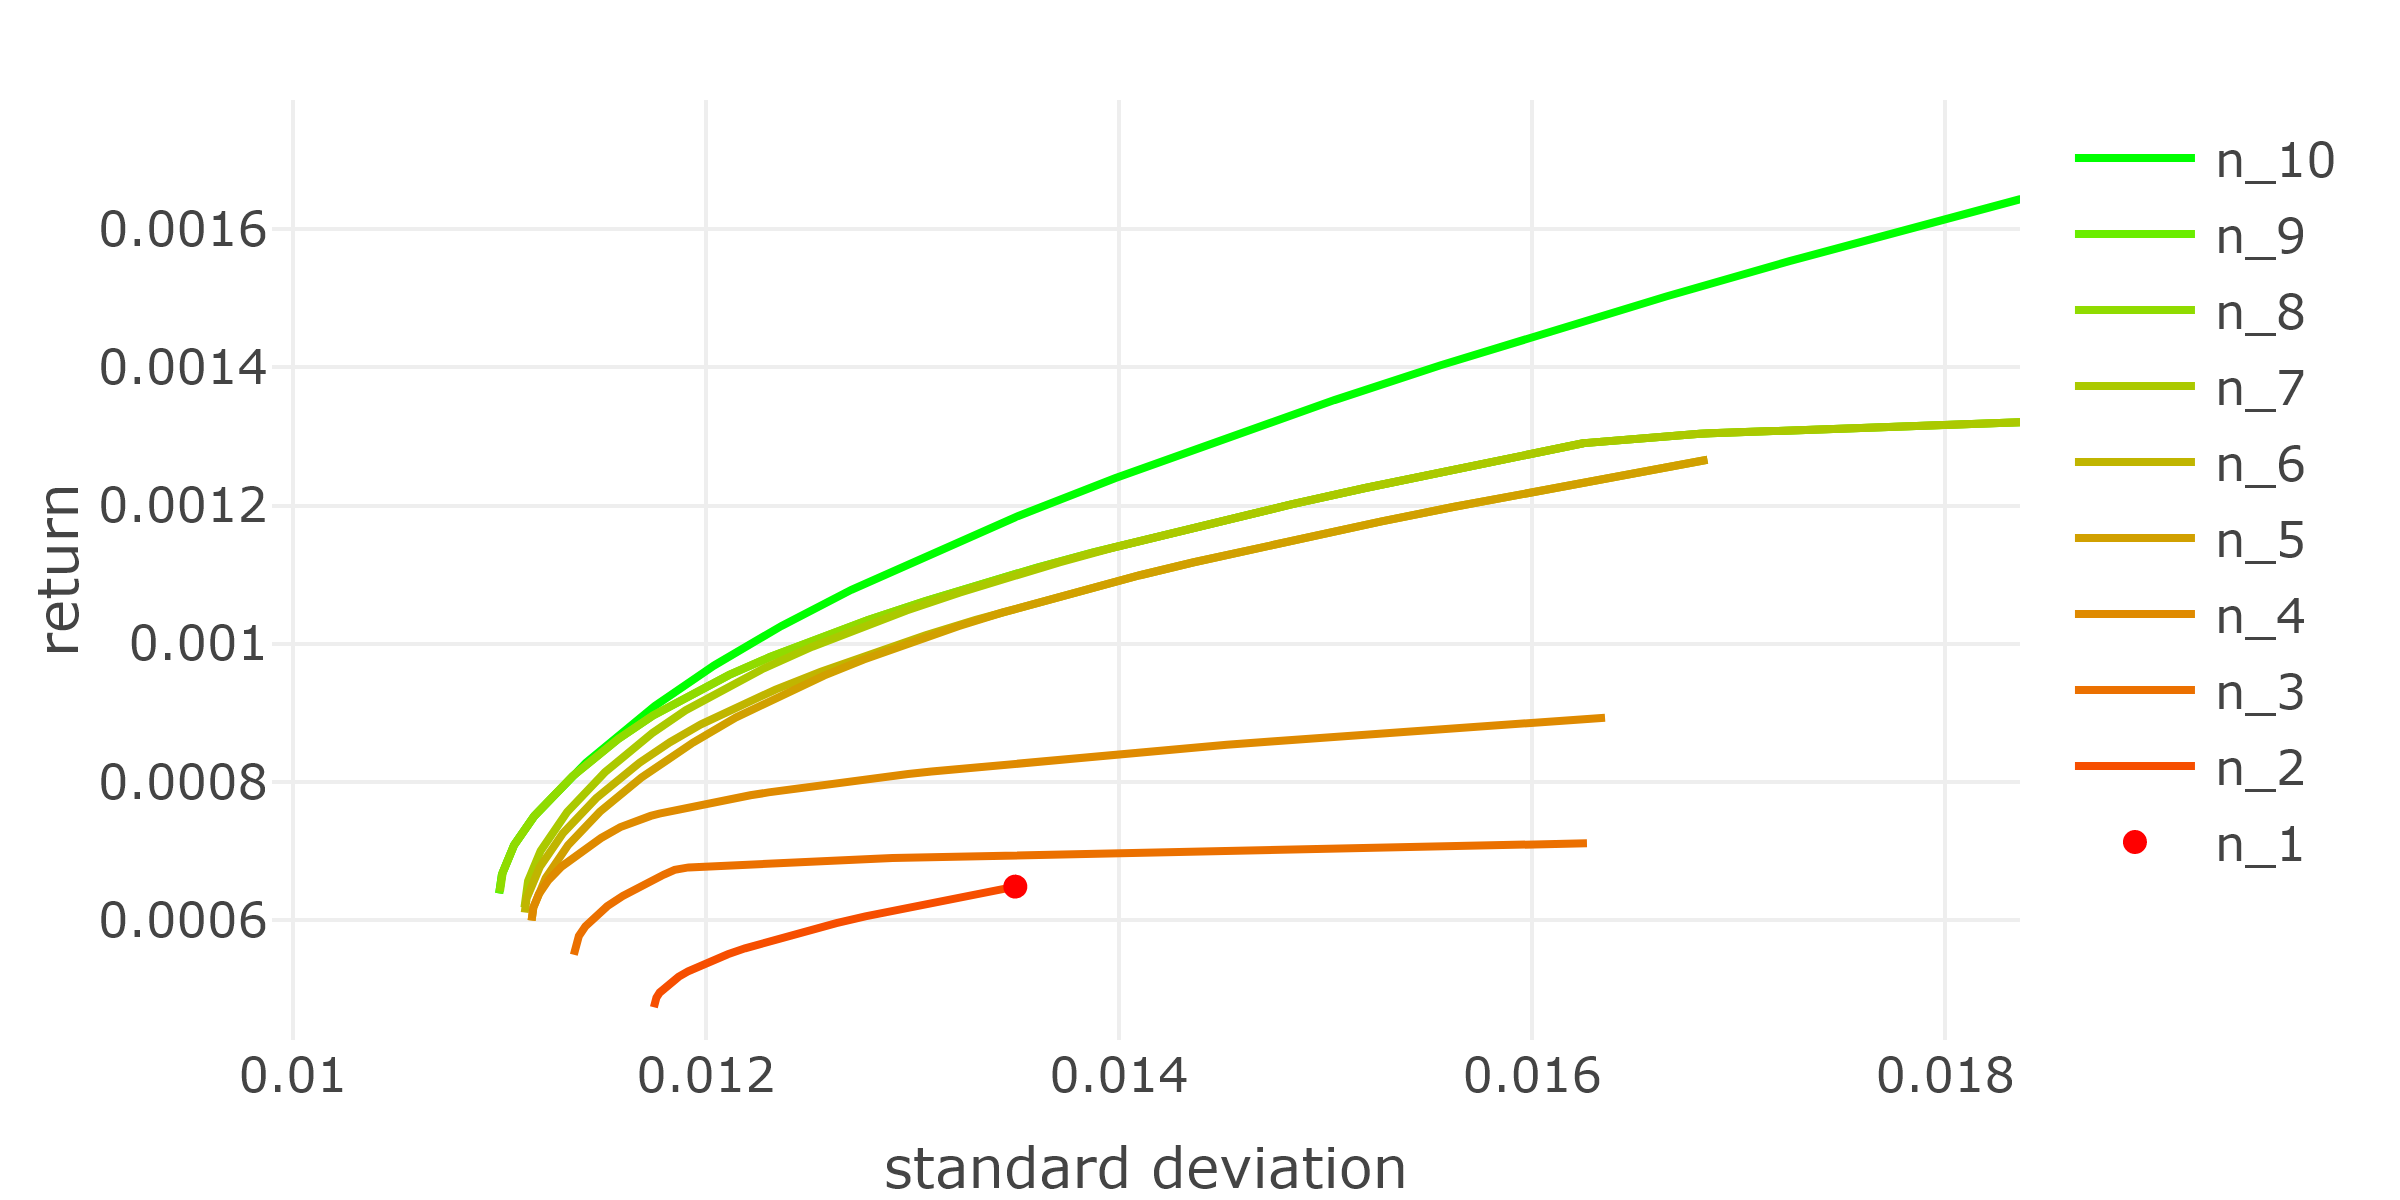
\includegraphics{Master_Thesis_files/figure-latex/unnamed-chunk-16-1.png}

It can be seen, that each asset added results in a minimum variance portfolio with smaller or equal standard deviation. Nonetheless that it started with the asset that has the smallest standard deviation of 0.0134977. This is the effect of diversification mentioned by Markowitz.

\hypertarget{example-solving-itp-with-solve.qp}{%
\section{\texorpdfstring{Example: Solving ITP with \texttt{solve.QP()}}{Example: Solving ITP with solve.QP()}}\label{example-solving-itp-with-solve.qp}}

This example will analyse how many assets are needed to minimize the variance between the replication and the S\&P 500 historical returns from \texttt{2016-01-01} to \texttt{2021-12-31}. The constraints are set to be long only and the weights should sum up to one. To step-wise reduce the number of assets, the five assets with the least weights gets discarded and acts as the new asset pool for the next replication, until only five assets are left. At first the needed data can be downloaded with existing functions from the \texttt{R/} directory. The function \texttt{get\_spx\_composition()} uses web scrapping to read the constituents of \href{https://en.wikipedia.org/wiki/List_of_S\%26P_500_companies}{wikipedia} and transforms it in monthly compositions of the S\&P 500. The pool is created by all assets that are present in the last month of the timeframe, reduced by assets with missing values. The code below, loads returns of all assets in the pool and the S\&P 500:

\begin{Shaded}
\begin{Highlighting}[]
\NormalTok{from }\OtherTok{\textless{}{-}} \StringTok{"2016{-}01{-}01"}
\NormalTok{to }\OtherTok{\textless{}{-}} \StringTok{"2021{-}12{-}31"}

\NormalTok{spx\_composition }\OtherTok{\textless{}{-}} \FunctionTok{buffer}\NormalTok{(}
  \FunctionTok{get\_spx\_composition}\NormalTok{(),}
  \StringTok{"AS\_spx\_composition"}
\NormalTok{)}


\NormalTok{pool\_returns\_raw }\OtherTok{\textless{}{-}} \FunctionTok{buffer}\NormalTok{(}
  \FunctionTok{get\_yf}\NormalTok{(}
    \AttributeTok{tickers =}\NormalTok{ spx\_composition }\SpecialCharTok{\%\textgreater{}\%} 
      \FunctionTok{filter}\NormalTok{(Date}\SpecialCharTok{\textless{}=}\NormalTok{to) }\SpecialCharTok{\%\textgreater{}\%} 
      \FunctionTok{filter}\NormalTok{(Date}\SpecialCharTok{==}\FunctionTok{max}\NormalTok{(Date)) }\SpecialCharTok{\%\textgreater{}\%} 
      \FunctionTok{pull}\NormalTok{(Ticker), }
    \AttributeTok{from =}\NormalTok{ from, }
    \AttributeTok{to =}\NormalTok{ to}
\NormalTok{  )}\SpecialCharTok{$}\NormalTok{returns, }
  \StringTok{"AS\_sp500\_assets"}
\NormalTok{)}
\NormalTok{pool\_returns\_raw }\OtherTok{\textless{}{-}} 
\NormalTok{  pool\_returns\_raw[, }\FunctionTok{colSums}\NormalTok{(}\FunctionTok{is.na}\NormalTok{(pool\_returns\_raw))}\SpecialCharTok{==}\DecValTok{0}\NormalTok{]}


\NormalTok{bm\_returns }\OtherTok{\textless{}{-}} \FunctionTok{buffer}\NormalTok{(}
  \FunctionTok{get\_yf}\NormalTok{(}\AttributeTok{tickers =} \StringTok{"\%5EGSPC"}\NormalTok{, }\AttributeTok{from =}\NormalTok{ from, }\AttributeTok{to =}\NormalTok{ to)}\SpecialCharTok{$}\NormalTok{returns, }
  \StringTok{"AS\_sp500"}
\NormalTok{) }\SpecialCharTok{\%\textgreater{}\%} \FunctionTok{setNames}\NormalTok{(., }\StringTok{"S\&P 500"}\NormalTok{)}
\end{Highlighting}
\end{Shaded}

Now are all needed data present and the function for the ITP can be created. It needs \texttt{pool\_returns} with variable number of columns and the single column matrix \texttt{bm\_returns}.

\begin{Shaded}
\begin{Highlighting}[]
\NormalTok{itp }\OtherTok{\textless{}{-}} \ControlFlowTok{function}\NormalTok{(pool\_returns, bm\_returns)\{}
\NormalTok{  mat }\OtherTok{\textless{}{-}} \FunctionTok{list}\NormalTok{(}
    \AttributeTok{Dmat =} \FunctionTok{cov}\NormalTok{(pool\_returns),}
    \AttributeTok{dvec =} \FunctionTok{cov}\NormalTok{(pool\_returns, bm\_returns),}
    \AttributeTok{Amat =} \FunctionTok{t}\NormalTok{(}\FunctionTok{rbind}\NormalTok{(}
      \FunctionTok{rep}\NormalTok{(}\DecValTok{1}\NormalTok{, }\FunctionTok{ncol}\NormalTok{(pool\_returns)), }\CommentTok{\# sum up to 1}
      \FunctionTok{diag}\NormalTok{(}\DecValTok{1}\NormalTok{, }
           \AttributeTok{nrow=}\FunctionTok{ncol}\NormalTok{(pool\_returns), }
           \AttributeTok{ncol=}\FunctionTok{ncol}\NormalTok{(pool\_returns)) }\CommentTok{\# long only}
\NormalTok{    )),}
    \AttributeTok{bvec =} \FunctionTok{c}\NormalTok{(}
      \DecValTok{1}\NormalTok{, }\CommentTok{\# sum up to 1}
      \FunctionTok{rep}\NormalTok{(}\DecValTok{0}\NormalTok{, }\FunctionTok{ncol}\NormalTok{(pool\_returns)) }\CommentTok{\# long only}
\NormalTok{    ),}
    \AttributeTok{meq =} \DecValTok{1}
\NormalTok{  )}
  
\NormalTok{  qp }\OtherTok{\textless{}{-}} \FunctionTok{solve.QP}\NormalTok{(}
    \AttributeTok{Dmat =}\NormalTok{ mat}\SpecialCharTok{$}\NormalTok{Dmat, }\AttributeTok{dvec =}\NormalTok{ mat}\SpecialCharTok{$}\NormalTok{dvec, }
    \AttributeTok{Amat =}\NormalTok{ mat}\SpecialCharTok{$}\NormalTok{Amat, }\AttributeTok{bvec =}\NormalTok{ mat}\SpecialCharTok{$}\NormalTok{bvec, }\AttributeTok{meq =}\NormalTok{ mat}\SpecialCharTok{$}\NormalTok{meq}
\NormalTok{  )}

\NormalTok{  res }\OtherTok{\textless{}{-}} \FunctionTok{list}\NormalTok{(}
    \StringTok{"var"} \OtherTok{=} \FunctionTok{as.numeric}\NormalTok{(}
      \FunctionTok{var}\NormalTok{(pool\_returns }\SpecialCharTok{\%*\%}\NormalTok{ qp}\SpecialCharTok{$}\NormalTok{solution }\SpecialCharTok{{-}}\NormalTok{ bm\_returns)),}
    \StringTok{"solution"} \OtherTok{=} \FunctionTok{setNames}\NormalTok{(qp}\SpecialCharTok{$}\NormalTok{solution, }\FunctionTok{colnames}\NormalTok{(pool\_returns))}
\NormalTok{  )}
\NormalTok{\}}
\end{Highlighting}
\end{Shaded}

Now can the replication and successive discarding of assets begin. The results are saved in \texttt{res} and used to plot the results.

\begin{Shaded}
\begin{Highlighting}[]
\NormalTok{res }\OtherTok{\textless{}{-}} \ConstantTok{NULL}
\ControlFlowTok{for}\NormalTok{(i }\ControlFlowTok{in} \FunctionTok{rev}\NormalTok{(}\FunctionTok{seq}\NormalTok{(}\DecValTok{5}\NormalTok{, }\FunctionTok{ncol}\NormalTok{(pool\_returns\_raw), }\DecValTok{5}\NormalTok{)))\{}
  \ControlFlowTok{if}\NormalTok{(i}\SpecialCharTok{==}\FunctionTok{ncol}\NormalTok{(pool\_returns\_raw))\{}
\NormalTok{    temp }\OtherTok{\textless{}{-}} \FunctionTok{itp}\NormalTok{(pool\_returns\_raw, bm\_returns)}
\NormalTok{  \}}\ControlFlowTok{else}\NormalTok{\{}
\NormalTok{    temp }\OtherTok{\textless{}{-}} \FunctionTok{itp}\NormalTok{(pool\_returns\_raw[, }\FunctionTok{names}\NormalTok{(}\FunctionTok{sort}\NormalTok{(temp}\SpecialCharTok{$}\NormalTok{solution, }\AttributeTok{decreasing =}\NormalTok{ T)[}\DecValTok{1}\SpecialCharTok{:}\NormalTok{i])], bm\_returns)}
\NormalTok{  \}}
\NormalTok{  res }\OtherTok{\textless{}{-}} \FunctionTok{rbind}\NormalTok{(res, }\FunctionTok{data.frame}\NormalTok{(}\StringTok{"N"}\OtherTok{=}\NormalTok{i, }\StringTok{"var"}\OtherTok{=}\NormalTok{temp}\SpecialCharTok{$}\NormalTok{var, }\StringTok{"sd"}\OtherTok{=}\FunctionTok{sqrt}\NormalTok{(temp}\SpecialCharTok{$}\NormalTok{var), }\AttributeTok{row.names =} \ConstantTok{NULL}\NormalTok{))}
\NormalTok{\}}


\FunctionTok{plot\_ly}\NormalTok{(}\AttributeTok{data=}\NormalTok{res, }\AttributeTok{x=}\SpecialCharTok{\textasciitilde{}}\NormalTok{N, }\AttributeTok{y=}\SpecialCharTok{\textasciitilde{}}\NormalTok{sd, }\AttributeTok{mode=}\StringTok{"lines"}\NormalTok{, }\AttributeTok{type =} \StringTok{\textquotesingle{}scatter\textquotesingle{}}\NormalTok{) }\SpecialCharTok{\%\textgreater{}\%} 
  \FunctionTok{layout}\NormalTok{(}\AttributeTok{yaxis=}\FunctionTok{list}\NormalTok{(}\AttributeTok{range=}\FunctionTok{c}\NormalTok{(}\DecValTok{0}\NormalTok{, }\FunctionTok{mean}\NormalTok{(}\FunctionTok{max}\NormalTok{(res}\SpecialCharTok{$}\NormalTok{sd),}\FunctionTok{mean}\NormalTok{(res}\SpecialCharTok{$}\NormalTok{sd)) ))) }\SpecialCharTok{\%\textgreater{}\%} 
  \FunctionTok{html\_save}\NormalTok{()}
\end{Highlighting}
\end{Shaded}

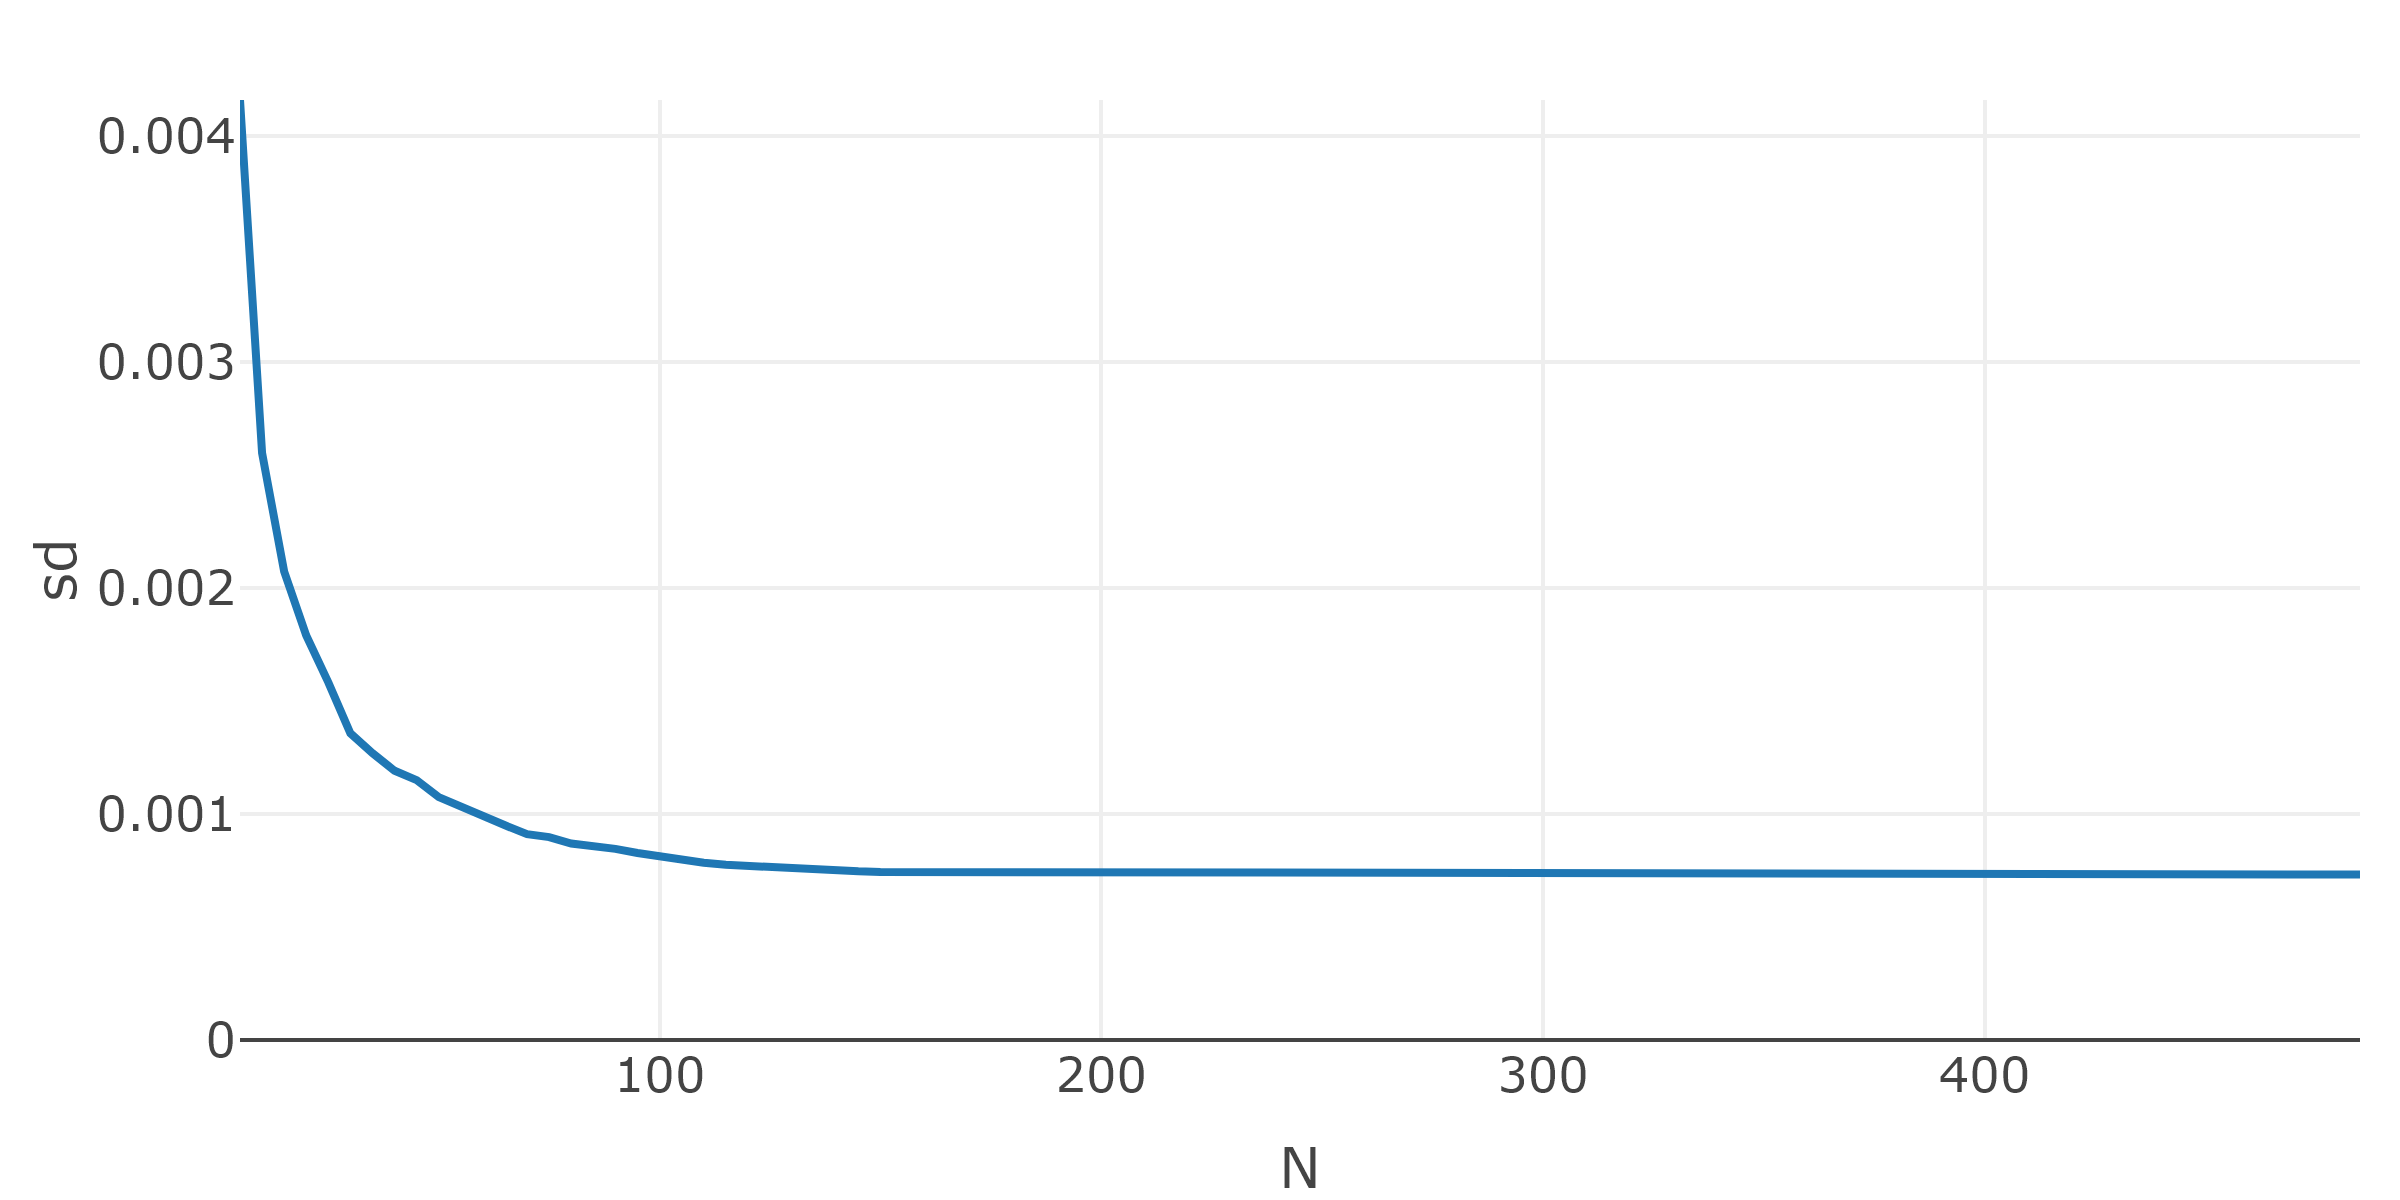
\includegraphics{Master_Thesis_files/figure-latex/unnamed-chunk-19-1.png}

It can be seen that the standard deviation stagnates at about \(N=100\). This results in the conclusion that a sparse replication with hundred assets is, in this specific case, sufficient to track the historical S\&P 500 performance of the timeframe.

\hypertarget{particle-swarm-optimization-pso}{%
\chapter{Particle Swarm Optimization (PSO)}\label{particle-swarm-optimization-pso}}

The PSO was developed by J. Kennedy as a Global Optimization method based on Swarm Intelligence and was introduced to the public in 1995 by Eberhart and Kennedy \citep{KeEb1995}. The initial PSO should resemble a flock of birds, that is flying through the sky without collisions. That is why its first applications were found in particle physics, to analyse moving particles in high dimensional spaces, which is resembled in the name Particle. Afterwards it was adapted in Evolutionary Computation to exploit a set of potential solutions in high dimensions and find the optima by cooperation with other particles in the swarm \citep{PaVr2002}. The benefits compared to some other Global Optimization methods are the fact that no gradient information is needed. It can find the optimum by considering only the result of the function that needs to be optimized. That means that the function can be arbitrarily complex and its still possible to reach the global optimum. Other benefits are the low computational costs, because only basic mathematical operators are used.

\hypertarget{the-algorithm}{%
\section{The Algorithm}\label{the-algorithm}}

Each Particle \(d\) with position \(x_d\) moves in the search space \(R^N\) and has its inherent velocity \(v_d\) and remembers its previous best position \(P_d\). After each iteration the velocity changes into the direction of its inherent velocity, its best previous position and the global best position \(p_g\) of all particles. A position change from \(i\) to \(i+1\) can be calculated by the following two equations \citep{PaVr2002}:

\begin{align*}
  v_d^{i+1} &= wv_d^{i} + c_p r_1^i (P_d^i-x_d^i) + c_g r_2^i (p_g^i - x_d^i) \\
  x_d^{i+1} &= x_d^i + v_d^{i+1}
\end{align*}

with \(r_1\) and \(r_2\) being uniformly distributed random numbers in {[}0, 1{]}. The cognitive parameter \(c_p\) acts as the weighting of the direction to its previous best position of the particle. On the contrary is the social parameter \(c_g\), which is a weighting to the direction of the global best position. The inertia weight \(w\) is crucial for the convergence behavior by remembering a part of its previous trajectory. A study examined in \citep{PaVr2002} showed that these parameters can be set to \(c_p=c_g=0.5\) and \(w\) should decrease from \(1.2\) to \(0\). However, some problems do benefit from more fine-tuning of these parameters. To provide a effortless translation to code, the formula above can be stated for \(d = 1, 2, \cdots, D\) particles in the following matrix notation:
\[
  V^{i+1} = w \cdot V^{i} + c_1 \cdot r_1^i \cdot (P^i-X^i) + c_2 \cdot r_2^i \cdot (p_g^i - X^i) \\
  X^{i+1} = X^i + V^{i+1}
\]
with current positions \(X \in R^{N \times D}\), current velocity's \(V \in R^{N \times D}\), previous best positions \(P \in R^{N \times D}\) and the global best position \(p_g \in R^{N}\). The parameters \(w\), \(c_p\), \(c_g\), \(r_1\) and \(r_2\) are stile scalars.

\hypertarget{pso-function}{%
\section{\texorpdfstring{\texttt{pso()} Function}{pso() Function}}\label{pso-function}}

A general purpose PSO function is created in this section by following the structure of other optimization heuristics in R, specially the existing PSO implementation from the R-Package \texttt{pso}. The center of everything is a objective function \texttt{fn()} which will return a scalar that needs to be minimized. The function itself needs mainly a vector \texttt{pos} that describes the position of a particle (e.g.~weights). The other main parameters for the PSO function are \texttt{par}, which is one position of a particle, that is used to derive the dimension of the problem and used as first position of one particle. The argument can contain only \texttt{NA}'s which results in completely randomized starting positions. The last two arguments needed are \texttt{lower} and \texttt{upper} bounds (e.g.~weights bigger than 0 and smaller than 1). All other parameters have default values that can be overwritten by passing a list named \texttt{control}. The resulting structure is:

\begin{Shaded}
\begin{Highlighting}[]
\NormalTok{pso }\OtherTok{\textless{}{-}} \ControlFlowTok{function}\NormalTok{(}
\NormalTok{    par, }
\NormalTok{    fn, }
\NormalTok{    lower, }
\NormalTok{    upper, }
    \AttributeTok{control =} \FunctionTok{list}\NormalTok{()}
\NormalTok{  )\{}

\NormalTok{\}}
\end{Highlighting}
\end{Shaded}

Before the main data-structure can be initialized, its necessary to create some example inputs for the \texttt{pso()} function like below:

\begin{Shaded}
\begin{Highlighting}[]
\NormalTok{par }\OtherTok{\textless{}{-}} \FunctionTok{rep}\NormalTok{(}\ConstantTok{NA}\NormalTok{, }\DecValTok{2}\NormalTok{)}
\NormalTok{fn }\OtherTok{\textless{}{-}} \ControlFlowTok{function}\NormalTok{(x)\{}\FunctionTok{return}\NormalTok{(}\FunctionTok{sum}\NormalTok{(}\FunctionTok{abs}\NormalTok{(x)))\}}
\NormalTok{lower }\OtherTok{\textless{}{-}} \SpecialCharTok{{-}}\DecValTok{10}
\NormalTok{upper }\OtherTok{\textless{}{-}} \DecValTok{10}
\NormalTok{control }\OtherTok{=} \FunctionTok{list}\NormalTok{(}
  \AttributeTok{s =} \DecValTok{10}\NormalTok{, }\CommentTok{\# swarm size}
  \AttributeTok{c.p =} \FloatTok{0.5}\NormalTok{, }\CommentTok{\# inherit best}
  \AttributeTok{c.g =} \FloatTok{0.5}\NormalTok{, }\CommentTok{\# global best}
  \AttributeTok{maxiter =} \DecValTok{100}\NormalTok{, }\CommentTok{\# iterations}
  \AttributeTok{w0 =} \FloatTok{1.2}\NormalTok{, }\CommentTok{\# starting inertia weight}
  \AttributeTok{wN =} \DecValTok{0}\NormalTok{, }\CommentTok{\# ending inertia weight}
  \AttributeTok{save\_traces =}\NormalTok{ F }\CommentTok{\# save more information}
\NormalTok{)}
\end{Highlighting}
\end{Shaded}

Now is the time to initialize the random positions \texttt{X}, its fitness \texttt{X\_fit} and its random velocity's \texttt{V} with the function \texttt{mrunif()}, which will create a matrix from uniformly distributed random numbers between \texttt{lower} and \texttt{upper}:

\begin{Shaded}
\begin{Highlighting}[]
\NormalTok{X }\OtherTok{\textless{}{-}} \FunctionTok{mrunif}\NormalTok{(}
  \AttributeTok{nr =} \FunctionTok{length}\NormalTok{(par), }\AttributeTok{nc=}\NormalTok{control}\SpecialCharTok{$}\NormalTok{s, }\AttributeTok{lower=}\NormalTok{lower, }\AttributeTok{upper=}\NormalTok{upper}
\NormalTok{)}
\ControlFlowTok{if}\NormalTok{(}\FunctionTok{all}\NormalTok{(}\SpecialCharTok{!}\FunctionTok{is.na}\NormalTok{(par)))\{}
\NormalTok{  X[, }\DecValTok{1}\NormalTok{] }\OtherTok{\textless{}{-}}\NormalTok{ par}
\NormalTok{\}}
\NormalTok{X\_fit }\OtherTok{\textless{}{-}} \FunctionTok{apply}\NormalTok{(X, }\DecValTok{2}\NormalTok{, fn)}
\NormalTok{V }\OtherTok{\textless{}{-}} \FunctionTok{mrunif}\NormalTok{(}
  \AttributeTok{nr =} \FunctionTok{length}\NormalTok{(par), }\AttributeTok{nc=}\NormalTok{control}\SpecialCharTok{$}\NormalTok{s, }
  \AttributeTok{lower=}\SpecialCharTok{{-}}\NormalTok{(upper}\SpecialCharTok{{-}}\NormalTok{lower), }\AttributeTok{upper=}\NormalTok{(upper}\SpecialCharTok{{-}}\NormalTok{lower)}
\NormalTok{)}\SpecialCharTok{/}\DecValTok{4}
\end{Highlighting}
\end{Shaded}

The velocity's are compressed with factor 4 to start with a maximal movement from a quarter of the space in each axis. The personal best positions \texttt{P} are the same as \texttt{X} and the global best position is the position with the smallest fitness:

\begin{Shaded}
\begin{Highlighting}[]
\NormalTok{P }\OtherTok{\textless{}{-}}\NormalTok{ X}
\NormalTok{P\_fit }\OtherTok{\textless{}{-}}\NormalTok{ X\_fit}
\NormalTok{p\_g }\OtherTok{\textless{}{-}}\NormalTok{ P[, }\FunctionTok{which.min}\NormalTok{(P\_fit)]}
\NormalTok{p\_g\_fit }\OtherTok{\textless{}{-}} \FunctionTok{which.min}\NormalTok{(P\_fit)}
\end{Highlighting}
\end{Shaded}

The needed data-structure is present and the optimization can start by calculating the new velocity's and the transformation of the old positions. If particles have left the valid space, they get pushed back to the border. Afterwards the fitness is calculated and the personal best and global best positions are saved, if they have improved.

\begin{Shaded}
\begin{Highlighting}[]
\NormalTok{trace\_data }\OtherTok{\textless{}{-}} \ConstantTok{NULL}
\ControlFlowTok{for}\NormalTok{(i }\ControlFlowTok{in} \DecValTok{1}\SpecialCharTok{:}\NormalTok{control}\SpecialCharTok{$}\NormalTok{maxiter)\{}
  \CommentTok{\# move particles}
\NormalTok{  V }\OtherTok{\textless{}{-}} 
\NormalTok{    (control}\SpecialCharTok{$}\NormalTok{w0}\SpecialCharTok{{-}}\NormalTok{(control}\SpecialCharTok{$}\NormalTok{w0}\SpecialCharTok{{-}}\NormalTok{control}\SpecialCharTok{$}\NormalTok{wN)}\SpecialCharTok{*}\NormalTok{i}\SpecialCharTok{/}\NormalTok{control}\SpecialCharTok{$}\NormalTok{maxiter) }\SpecialCharTok{*}\NormalTok{ V }\SpecialCharTok{+} 
\NormalTok{    control}\SpecialCharTok{$}\NormalTok{c.p }\SpecialCharTok{*} \FunctionTok{runif}\NormalTok{(}\DecValTok{1}\NormalTok{) }\SpecialCharTok{*}\NormalTok{ (P}\SpecialCharTok{{-}}\NormalTok{X) }\SpecialCharTok{+} 
\NormalTok{    control}\SpecialCharTok{$}\NormalTok{c.g }\SpecialCharTok{*} \FunctionTok{runif}\NormalTok{(}\DecValTok{1}\NormalTok{) }\SpecialCharTok{*}\NormalTok{ (p\_g}\SpecialCharTok{{-}}\NormalTok{X)}
\NormalTok{  X }\OtherTok{\textless{}{-}}\NormalTok{ X }\SpecialCharTok{+}\NormalTok{ V}
  
  \CommentTok{\# set velocity to zeros if not in valid space}
\NormalTok{  V[X }\SpecialCharTok{\textgreater{}}\NormalTok{ upper] }\OtherTok{\textless{}{-}} \DecValTok{0}
\NormalTok{  V[X }\SpecialCharTok{\textless{}}\NormalTok{ lower] }\OtherTok{\textless{}{-}} \DecValTok{0}
  
  \CommentTok{\# move into valid space}
\NormalTok{  X[X }\SpecialCharTok{\textgreater{}}\NormalTok{ upper] }\OtherTok{\textless{}{-}}\NormalTok{ upper}
\NormalTok{  X[X }\SpecialCharTok{\textless{}}\NormalTok{ lower] }\OtherTok{\textless{}{-}}\NormalTok{ lower}
  
  \CommentTok{\# evaluate objective function}
\NormalTok{  X\_fit }\OtherTok{\textless{}{-}} \FunctionTok{apply}\NormalTok{(X, }\DecValTok{2}\NormalTok{, fn)}
  
  \CommentTok{\# save new previews best}
\NormalTok{  P[, P\_fit }\SpecialCharTok{\textgreater{}}\NormalTok{ X\_fit] }\OtherTok{\textless{}{-}}\NormalTok{ X[, P\_fit }\SpecialCharTok{\textgreater{}}\NormalTok{ X\_fit]}
\NormalTok{  P\_fit[P\_fit }\SpecialCharTok{\textgreater{}}\NormalTok{ X\_fit] }\OtherTok{\textless{}{-}}\NormalTok{ X\_fit[P\_fit }\SpecialCharTok{\textgreater{}}\NormalTok{ X\_fit]}
  
  \CommentTok{\# save new global best}
  \ControlFlowTok{if}\NormalTok{(}\FunctionTok{any}\NormalTok{(P\_fit }\SpecialCharTok{\textless{}}\NormalTok{ p\_g\_fit))\{}
\NormalTok{    p\_g }\OtherTok{\textless{}{-}}\NormalTok{ P[, }\FunctionTok{which.min}\NormalTok{(P\_fit)]}
\NormalTok{    p\_g\_fit }\OtherTok{\textless{}{-}} \FunctionTok{min}\NormalTok{(P\_fit)}
\NormalTok{  \}}
  
  \ControlFlowTok{if}\NormalTok{(control}\SpecialCharTok{$}\NormalTok{save\_traces}\SpecialCharTok{==}\ConstantTok{TRUE}\NormalTok{)\{}
\NormalTok{    trace\_data }\OtherTok{\textless{}{-}} \FunctionTok{rbind}\NormalTok{(trace\_data, }\FunctionTok{data.frame}\NormalTok{(}\StringTok{"iter"}\OtherTok{=}\NormalTok{i, }\FunctionTok{t}\NormalTok{(X)))}
\NormalTok{  \}}
\NormalTok{\}}
\end{Highlighting}
\end{Shaded}

The best fitness after \(100\) iterations is 0.0000009 and the best possible solution is at \(0\).

\hypertarget{animation-2-dimensional}{%
\section{Animation 2-Dimensional}\label{animation-2-dimensional}}

This section provides insights into the behavior of the PSO by visualizing multiple iterations in a GIF. The GIF only works in Adobe Acrobat DC or in the Markdown/HTML Version of this thesis. The amazing template of the animation is inspired by \href{https://www.r-bloggers.com/2021/10/how-to-build-a-basic-particle-swarm-optimiser-from-scratch-in-r/}{R'tichoke}. The PSO core from the chapter above was used to finish the \texttt{pso()} function and is used here with seed 0. The fucntion \texttt{fn} to evaluate is they same function as in \href{https://www.r-bloggers.com/2021/10/how-to-build-a-basic-particle-swarm-optimiser-from-scratch-in-r/}{R'tichoke}.

\begin{Shaded}
\begin{Highlighting}[]
\FunctionTok{set.seed}\NormalTok{(}\DecValTok{0}\NormalTok{)}

\NormalTok{fn }\OtherTok{\textless{}{-}} \ControlFlowTok{function}\NormalTok{(pos)\{}
  \SpecialCharTok{{-}}\DecValTok{20} \SpecialCharTok{*} \FunctionTok{exp}\NormalTok{(}\SpecialCharTok{{-}}\FloatTok{0.2} \SpecialCharTok{*} \FunctionTok{sqrt}\NormalTok{(}\FloatTok{0.5} \SpecialCharTok{*}\NormalTok{((pos[}\DecValTok{1}\NormalTok{]}\SpecialCharTok{{-}}\DecValTok{1}\NormalTok{)}\SpecialCharTok{\^{}}\DecValTok{2} \SpecialCharTok{+}\NormalTok{ (pos[}\DecValTok{2}\NormalTok{]}\SpecialCharTok{{-}}\DecValTok{1}\NormalTok{)}\SpecialCharTok{\^{}}\DecValTok{2}\NormalTok{))) }\SpecialCharTok{{-}} 
  \FunctionTok{exp}\NormalTok{(}\FloatTok{0.5}\SpecialCharTok{*}\NormalTok{(}\FunctionTok{cos}\NormalTok{(}\DecValTok{2}\SpecialCharTok{*}\NormalTok{pi}\SpecialCharTok{*}\NormalTok{pos[}\DecValTok{1}\NormalTok{]) }\SpecialCharTok{+} \FunctionTok{cos}\NormalTok{(}\DecValTok{2}\SpecialCharTok{*}\NormalTok{pi}\SpecialCharTok{*}\NormalTok{pos[}\DecValTok{2}\NormalTok{]))) }\SpecialCharTok{+} 
  \FunctionTok{exp}\NormalTok{(}\DecValTok{1}\NormalTok{) }\SpecialCharTok{+} \DecValTok{20}
\NormalTok{\}}

\NormalTok{res }\OtherTok{\textless{}{-}} \FunctionTok{pso}\NormalTok{(}
  \AttributeTok{par =} \FunctionTok{rep}\NormalTok{(}\ConstantTok{NA}\NormalTok{, }\DecValTok{2}\NormalTok{),}
  \AttributeTok{fn =}\NormalTok{ fn,}
  \AttributeTok{lower =} \SpecialCharTok{{-}}\DecValTok{10}\NormalTok{,}
  \AttributeTok{upper =} \DecValTok{10}\NormalTok{,}
  \AttributeTok{control =} \FunctionTok{list}\NormalTok{(}
    \AttributeTok{s =} \DecValTok{10}\NormalTok{,}
    \AttributeTok{maxiter =} \DecValTok{30}\NormalTok{,}
    \AttributeTok{w0 =} \FloatTok{0.8}\NormalTok{,}
    \AttributeTok{save\_traces =}\NormalTok{ T}
\NormalTok{  )}
\NormalTok{)}
\end{Highlighting}
\end{Shaded}

The function \texttt{fn} has many local minima and a global minima at \((1,1)\) with value \(0\). The background-color-scale ranges from 0 as red to 20 as purple. The PSO has 10 particles, iterates 30 times with inertia weight decreasing from 0.8 to 0. The iterations are visualized in the GIF below:

\animategraphics[loop, width=8cm]{10}{./gifs/pso_2dim/gganim_plot}{1}{50}

\hypertarget{example-mvp}{%
\section{Example MVP}\label{example-mvp}}

This example uses the \texttt{solve.QP} approach from \ref{exampleanalyticalmvp} with ten assets as benchmark. Recap, the goal is to create a MVP from ten of the biggest american equity's between 2016 and 2021 for each possible \(\lambda\). The PSO has 100 particles and 200 iterations for each lambda. The key features of all portfolios generated with the \texttt{solve.QP} versus the PSO is shown below:
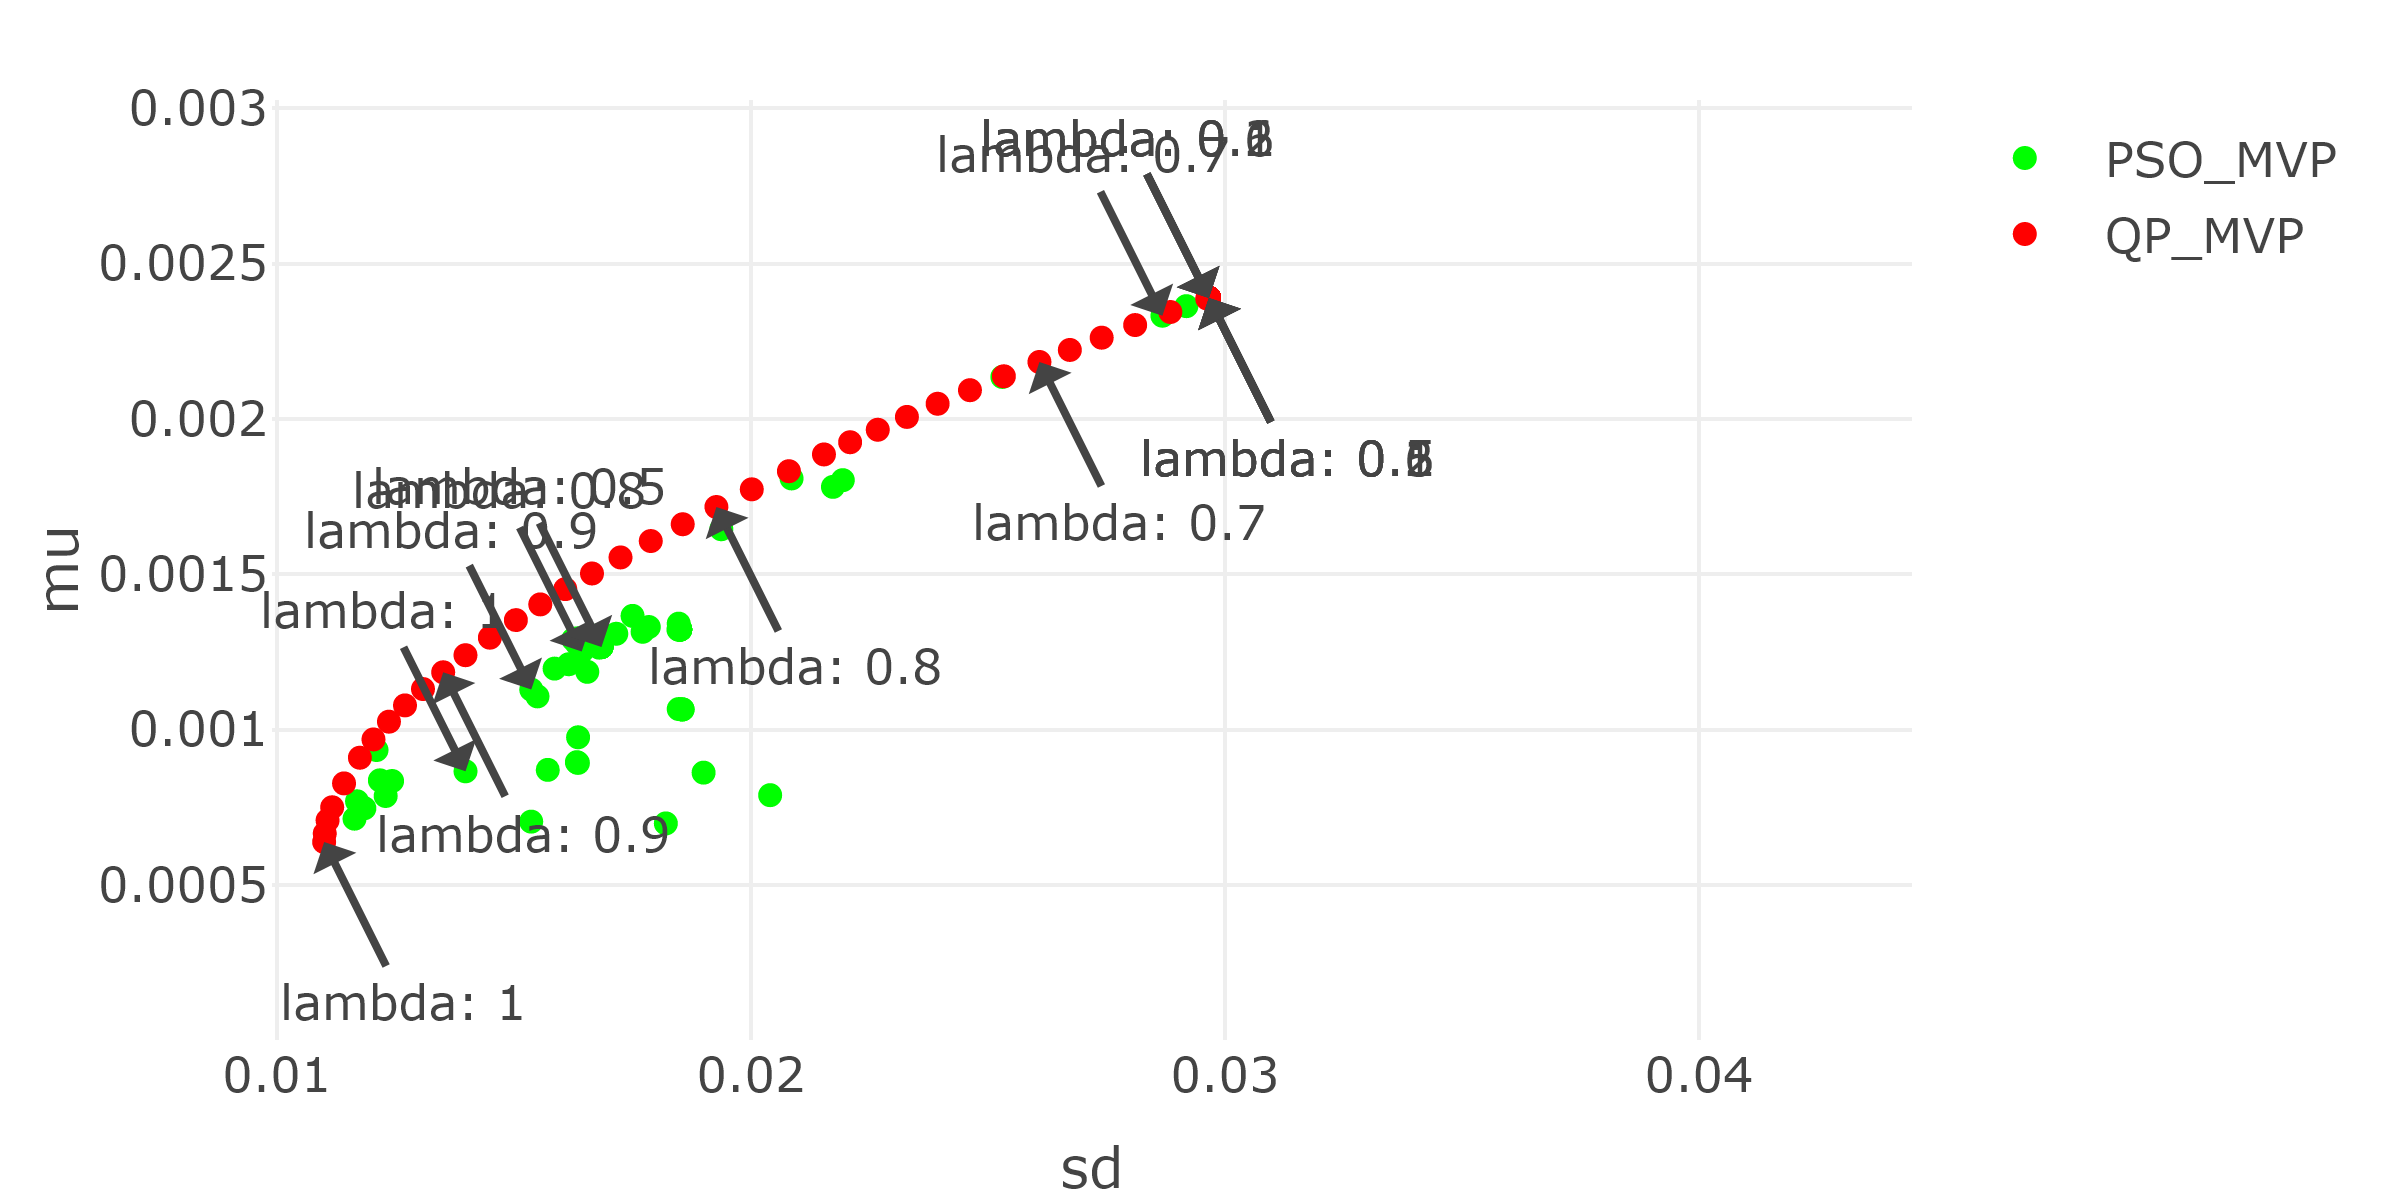
\includegraphics{Master_Thesis_files/figure-latex/unnamed-chunk-26-1.png}
It can be seen that the analytical approach and the PSO approach have a tiny difference for \(lambda > 0.9\) and a steadily increased difference otherwise. This indicates that minimum variance portfolios are more stable to generate with the PSO.

\hypertarget{example-itp-1}{%
\section{Example ITP}\label{example-itp-1}}

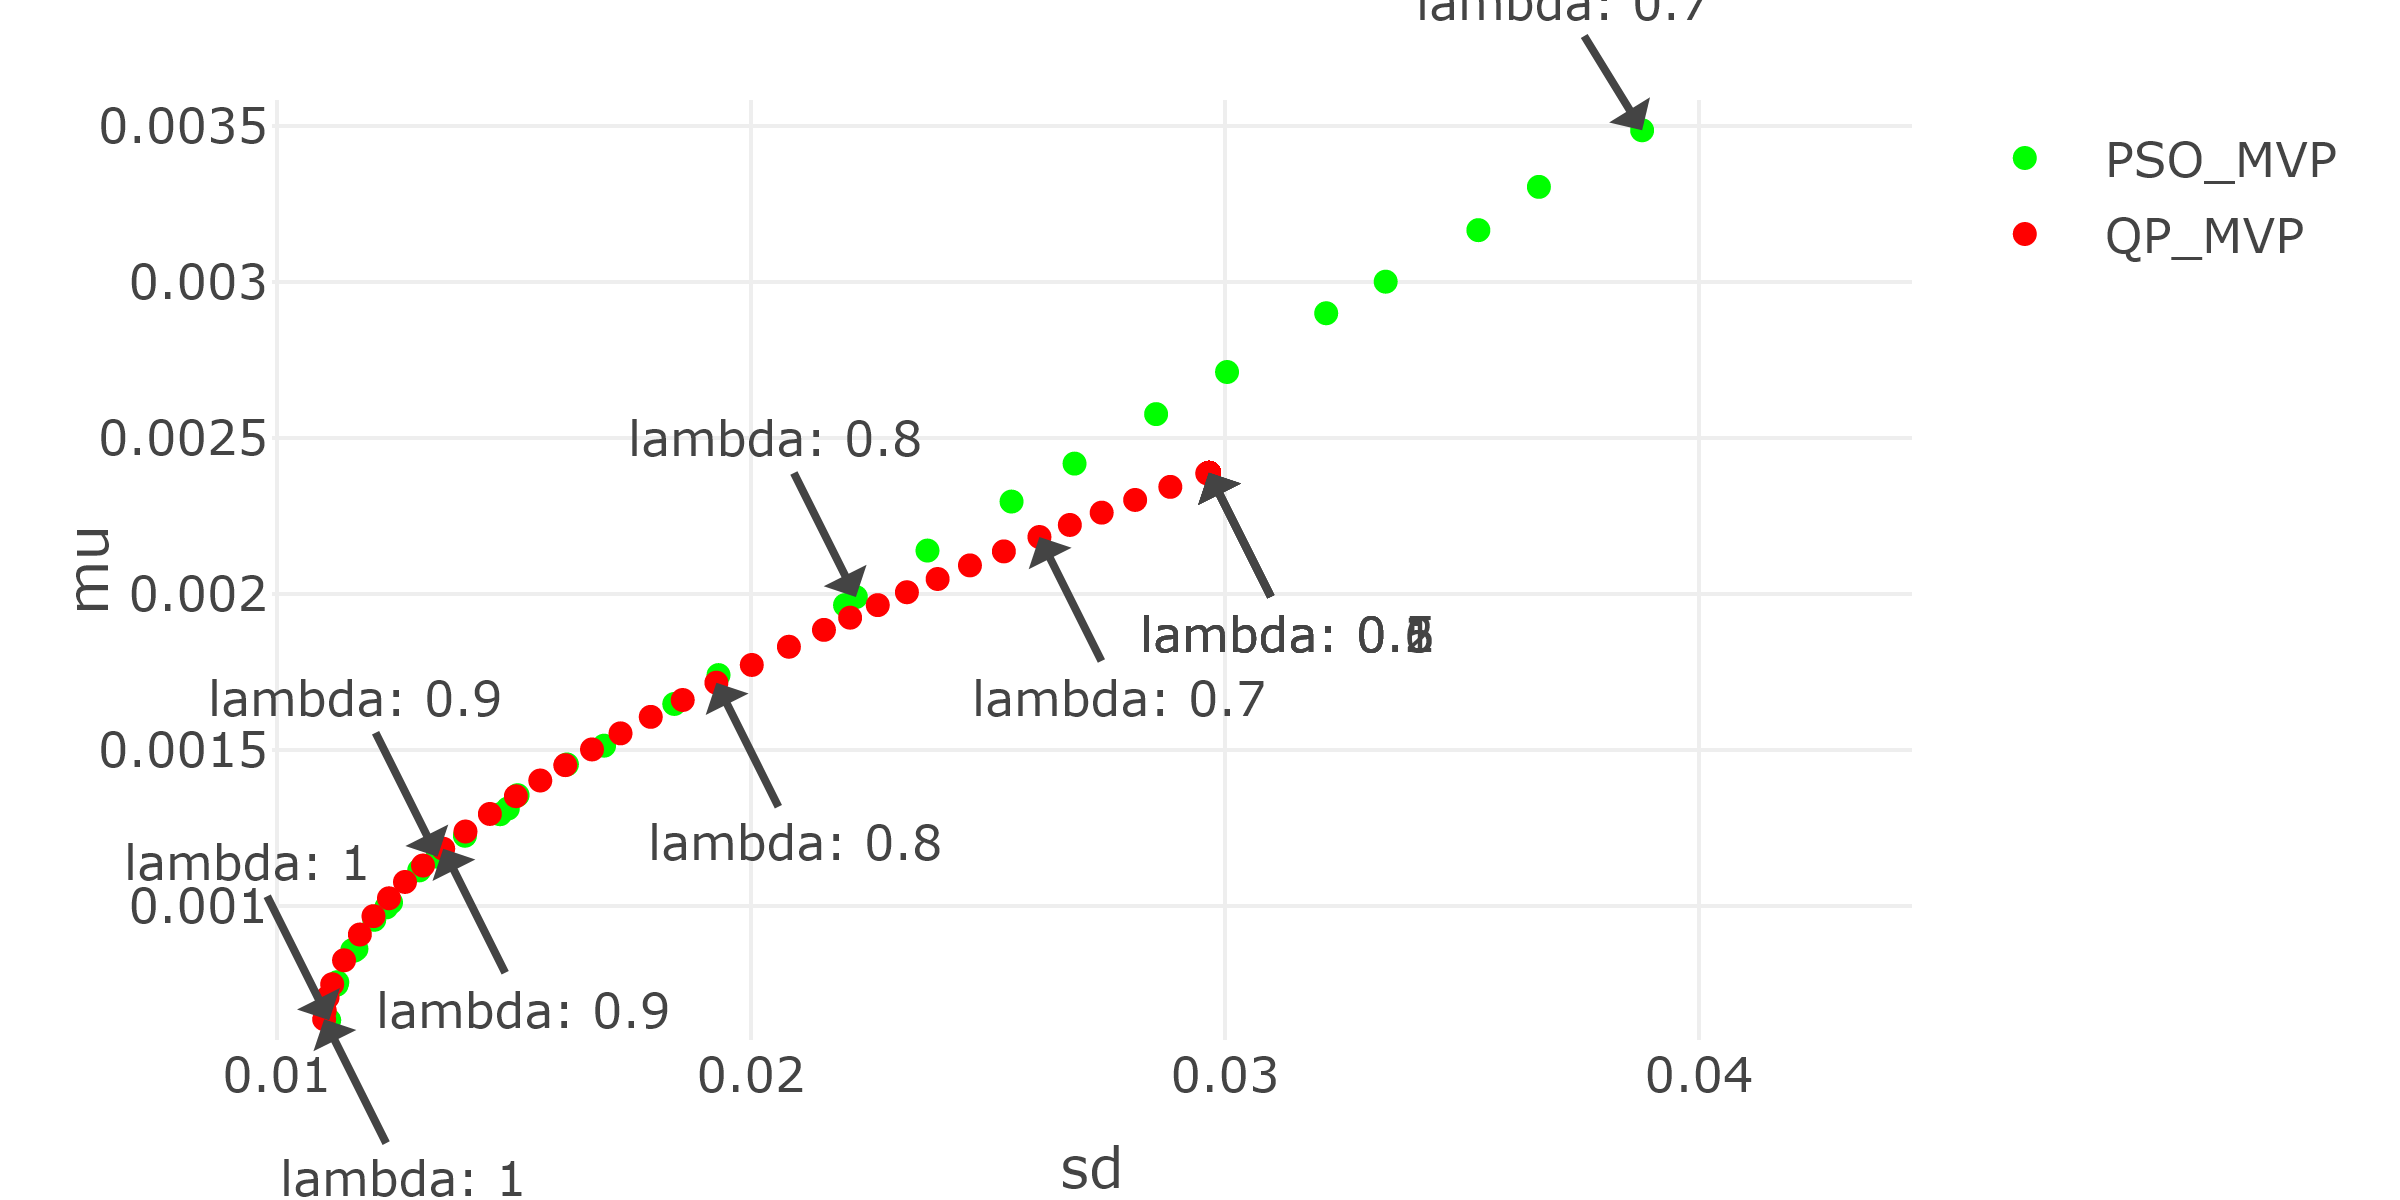
\includegraphics{Master_Thesis_files/figure-latex/unnamed-chunk-27-1.png}
The mean fitness

\hypertarget{pros-and-cons}{%
\section{Pros and Cons}\label{pros-and-cons}}

\hypertarget{functions}{%
\section{Functions}\label{functions}}

  \bibliography{book.bib,packages.bib}

\end{document}
